% (c) 2012 - 2014 Dimitrios Vrettos - d.vrettos@gmail.com
% (c) 2014 Claudio Carboncini - claudio.carboncini@gmail.com
\chapter{Identità, equazioni, equivalenza}
\section{Identità ed equazioni}

Analizziamo le seguenti proposizioni:

\begin{enumeratea}
\item ``cinque è uguale alla differenza tra sette e due'';
\item ``la somma di quattro e due è uguale a otto'';
\item ``il doppio di un numero naturale è uguale alla differenza tra nove e il numero stesso'';
\item ``la somma di due numeri interi è uguale a dieci''.
\end{enumeratea}

Notiamo che sono tutte costruite con il predicato
``essere uguale a''. Riscriviamo in formula ciascuna di esse:
\begin{multicols}{4}
 \begin{enumeratea}
\item $5=7-2$;
\item $4+2=8$;
\item $2x=9-x$;
\item $x+y=10$.
\end{enumeratea}
\end{multicols}
Notiamo che le prime due contengono solamente numeri, le seconde
contengono anche variabili (lettere).

Le formule del primo tipo si dicono \emph{chiuse} e
di esse si può subito stabilire se sono vere o false; così in~$\insN$ la
formula~$5 = 7 - 2$ è vera, mentre~$4 + 2 = 8$ è falsa.

\begin{definizione}
 Le \emph{formule chiuse} costruite con il predicato
<<essere uguale>> si chiamano \emph{uguaglianze};
definito l'ambiente in cui vengono enunciate si può
immediatamente stabilire il loro valore di verità.
\end{definizione}

\begin{exrig}
 \begin{esempio}
 La formula chiusa~$1 - 6 = -5$ è un'uguaglianza
vera se la consideriamo nell'insieme~$\insZ$ degli interi
relativi, è falsa se la vediamo come sottrazione tra numeri naturali.
 \end{esempio}
\end{exrig}

Le formule c) e d) che contengono variabili si dicono \emph{aperte}; le variabili che compaiono sono chiamate
\emph{incognite}. Di tali formule non si può subito stabilire il valore di verità.

Quando alle incognite sostituiamo un numero, queste si trasformano in
formule chiuse e allora possiamo stabilirne il valore di verità
relativamente alla sostituzione effettuata.

\begin{exrig}
 \begin{esempio}
 Nella formula~$2x = 9 - x$ sostituiamo alla variabile~$x$ il valore $0$; quindi otteniamo:~$2\cdot 0=9-0 \Rightarrow~0=9$, falsa.

 Sostituiamo ora alla
variabile~$x$ il valore $3$; otteniamo~$2\cdot 3=9-3 \Rightarrow~6=6$, vera.
 \end{esempio}

 \begin{esempio}
 Nella formula~$x + y = 10$ sostituiamo
alle variabili coppie di numeri interi come~$x = 2$ e~$y = 5$; otteniamo~$2+5=10\Rightarrow~7= 10$, falsa. Se
sostituiamo~$x = 4$ e~$y = 6$ ci rendiamo subito conto che
l'uguaglianza ottenuta è vera. Esistono
molte altre coppie di numeri interi che rendono vera
l'uguaglianza.
 \end{esempio}
\end{exrig}

\begin{definizione}
 Le formule aperte costruite con il predicato essere uguale si chiamano
\emph{equazioni}; le due espressioni che compaiono a sinistra e a
destra del segno di uguaglianza si chiamano rispettivamente
\emph{primo membro} e \emph{secondo membro}.

L'insieme dei valori che sostituiti alle incognite trasformano l'equazione in
un'uguaglianza vera costituisce
l'\emph{insieme soluzione} ($\IS$) o più semplicemente la \emph{soluzione} dell'equazione.
\end{definizione}

Affronteremo per ora equazioni in
\emph{una sola incognita} che, dopo aver svolto eventuali calcoli nei due membri, comparirà a
\emph{grado} 1 e i cui \emph{coefficienti} sono \emph{numeri razionali}.
Cercheremo la sua soluzione
nell'insieme~$\insQ$ dei numeri razionali, salvo esplicita indicazione differente.
\begin{exrig}
 \begin{esempio}
Cercare le soluzioni nell'insieme indicato.
 \begin{enumeratea}
 \item $x^{2}=1 \text{ con }x\in\insN.$
Risulta vera solo se a~$x$ sostituiamo il valore~1; infatti~1 è
l'unico numero naturale il cui quadrato è~1.
L'insieme soluzione è~$\{1\}$.
 \item $x^{2}=1 \text{ con }x\in\insZ$.
Risulta vera se a
$x$ sostituiamo il valore~1 oppure il valore~$-1$; infatti sia~$-1$ che~1
elevati al quadrato danno~1. L'insieme soluzione è
$\{-1\text{,~}1\}$.
 \item $x^{2}+1=0\text{ con }x\in\insR$.
Essendo la formula a sinistra
dell'uguale la somma di un quadrato con il numero~1, si ottiene sempre
un numero~$\geq1$ e non si può ottenere $0$, pertanto è impossibile trovare una soluzione, ovvero l'insieme soluzione è $\emptyset$.
 \item $2x+3=(3+x)+x \text{ con } x\in\insQ$.
Eseguendo il semplice calcolo al secondo
membro, ci rendiamo conto che qualunque valore venga sostituito
all'incognita l'uguaglianza risulta
vera. L'insieme soluzione è~$\insQ$.
\end{enumeratea}
 \end{esempio}
\end{exrig}

In generale un'equazione in una incognita può essere:

\begin{enumeratea}
\item \emph{determinata}, quando l'insieme soluzione è un sottoinsieme proprio
dell'insieme numerico considerato;
\item \emph{impossibile}, quando l'insieme soluzione è l'insieme vuoto~$\emptyset$;
\item \emph{indeterminata} o \emph{identità}, quando l'insieme soluzione coincide con
l'insieme considerato.
\end{enumeratea}

\begin{exrig}
 \begin{esempio}
 Analizziamo le equazioni:
\begin{multicols}{3}
 \begin{enumeratea}
 \item $3\cdot x=0$;
 \item $0\cdot x=5$;
 \item $0\cdot x=0$.
\end{enumeratea}
\end{multicols}

Tutte e tre hanno la stessa struttura: il primo membro è il prodotto
di un coefficiente numerico per un valore incognito, il secondo membro
è un numero.

\paragraph{a)} Per trovare l'insieme soluzione della prima equazione cerchiamo in~$\insQ$ il
numero che moltiplicato per~3 dà come prodotto~0. L'unico numero che rende vera
l'uguaglianza è zero. Quindi l'insieme delle soluzioni è~$\{0\}$. L'equazione è
determinata.

\paragraph{b)} Per trovare l'insieme soluzione della seconda equazione cerchiamo in~$\insQ$ il
numero che moltiplicato per~0 dà come prodotto~5. Per la proprietà
della moltiplicazione quando moltiplichiamo per~0 il prodotto è~0,
non otterremo mai~5. Quindi l'insieme soluzione è
l'insieme vuoto $\emptyset$. L'equazione è
impossibile.

\paragraph{c)} Per trovare l'insieme soluzione della terza equazione cerchiamo in~$\insQ$ il
numero che moltiplicato per zero dà come prodotto zero. Per la
proprietà della moltiplicazione quando moltiplichiamo per~0 il
prodotto è~0 qualunque sia l'altro fattore. Quindi
l'insieme delle soluzioni è~$\insQ$. L'equazione è
indeterminata.
 \end{esempio}
\end{exrig}

\subsection{Ricerca dell'insieme soluzione}
In alcuni casi la soluzione di un'equazione si può
trovare applicando semplicemente le proprietà delle operazioni.

\begin{exrig}
 \begin{esempio}
Analizziamo lo schema operativo dell'equazione~$3x-1=17 \text{ con } x\in\insN$.

Si opera sul valore incognito~$x$ per ottenere~17:

\[\text{\emph{entra} } x,\text{ si moltiplica per tre}\to~3\cdot x%
\text{ si sottrae } 1\to~3\cdot x-1 \text{ si ottiene } 17.\]

Qual è il valore in ingresso?

Per determinare il valore in ingresso basterà ripercorrere lo schema
 effettuando le operazioni inverse:
\[\text{\emph{da} } 17 \text{ aggiungi } 1\to~18 \text{ dividi per tre }\to~18:3 \to x.\]

La soluzione dell'equazione è~$x = 6$ e~$\IS$ (insieme
soluzione) è~$\{6\}$.
 \end{esempio}
\end{exrig}

\ovalbox{\risolvi \ref{ese:13.1}}\vspace{1.10ex}

Per risolvere un'equazione più complessa come
$\left(\dfrac{1}{2}x+3\right)\cdot (-5+x)=12x+\dfrac{1}{2}x^{2}$ con
$x\in~\insQ$, non possiamo applicare il procedimento precedente; potremmo
procedere per tentativi, sostituendo all'incognita
alcuni valori scelti a caso e verificando se il valore assunto dal
primo membro risulta uguale a quello assunto dal secondo membro. È
evidente però che questo procedimento raramente porterà a trovare
tutte le soluzioni di un'equazione.

\osservazione
Per risolvere un'equazione, cioè per determinare tutte
le eventuali soluzioni, si procede applicando i principi
d'equivalenza.

\section{Prinicipi di equivalenza}

\begin{definizione}
 Due equazioni sono \emph{equivalenti} se hanno lo stesso insieme soluzione.
\end{definizione}

\begin{principio}[Primo principio di equivalenza]
 Aggiungendo o sottraendo ad ambo i membri di
un'equazione data uno stesso numero o una stessa
espressione (definita per ogni valore dell'incognita)
si ottiene un'equazione equivalente a quella data.
\end{principio}

\begin{principio}[Secondo principio di equivalenza]
 Moltiplicando o dividendo ambo i membri di
un'equazione per uno stesso numero non nullo o per
un'espressione non nulla (definita per ogni valore
attribuito all'incognita) si ottiene
un'equazione equivalente alla data.
\end{principio}


La forma più semplice (forma canonica) di un'equazione di primo grado in
un'incognita è del tipo:
\[x = \text{ numero}.\]

L'insieme soluzione di una
equazione di questo tipo è semplicemente:
\[\IS=\{\text{numero}\}.\]

Per esempio, l'insieme delle soluzioni dell'equazione
$x = -3$ è~$\IS =\{-3\}$.

I principi sopra enunciati permettono di trasformare qualunque equazione
nella forma canonica che ha lo stesso insieme soluzione di quella
assegnata.

\subsection{Risoluzione di equazioni numeriche intere di primo grado}
In questo paragrafo vedremo come usare i principi
d'equivalenza prima enunciati per condurre
un'equazione alla forma canonica e dunque determinarne
la soluzione.

\begin{definizione}
\emph{Risolvere un'equazione} significa
determinare il suo Insieme Soluzione.
\end{definizione}

Cominciamo con alcuni esempi.

\begin{exrig}
 \begin{esempio}
Applicazione del~1{\textdegree} principio di equivalenza.

\begin{enumeratea}
\item $x-5=3$:
aggiungiamo~5 a entrambi i membri:~$x-5+5=3+5\:\Rightarrow\: x=8$, $\IS =\{8\}.$
\item $3x=2+2x$: sottraiamo~$2x$ a entrambi i membri:~$3x-2x=2+2x-2x\:\Rightarrow\: x=2$,
$\IS =\{2\}$.
\end{enumeratea}
 \end{esempio}
\end{exrig}

\ovalbox{\risolvii \ref{ese:13.2}, \ref{ese:13.3}, \ref{ese:13.4}, \ref{ese:13.5}}
\begin{exrig}
 \begin{esempio}
 Applicazione del~2{\textdegree} principio di equivalenza.

 \begin{enumeratea}
\item $3x=12$ dividiamo entrambi i membri per~3, si ha
\[\dfrac{3}{3}x=\dfrac{12}{3}\quad\Rightarrow\quad x=4\quad\to\quad\IS =\{4\}.\]
\item $\dfrac{1}{2}x=2$ moltiplichiamo entrambi i membri per~2, si ha
\[2\cdot {\dfrac{1}{2}}x=2\cdot 2\quad\Rightarrow\quad x=4\quad\to\quad\IS =\{4\}.\]
\end{enumeratea}
\end{esempio}
\end{exrig}

\ovalbox{\risolvii \ref{ese:13.6}, \ref{ese:13.7}, \ref{ese:13.8}}

%\newpage
 \begin{exrig}
 \begin{esempio}
 $-2x+1=3x-5$.

\begin{enumeratea}
 \item Sottraiamo~1 a entrambi i membri~$-2x+1-1=3x-5-1$ quindi~$-2x=3x-6$;
\item sottraiamo~$3x$ a entrambi i membri~$-2x-3x=3x-3x-6$ quindi~$-5x=-6$;
\item dividiamo entrambi i membri per~$-5$:~$\dfrac{-5}{-5}x=\dfrac{-6}{-5}\quad\Rightarrow\quad x=\dfrac{6}{5}\quad\rightarrow\quad
\IS =\left\{\dfrac{6}{5}\right\}.$
\end{enumeratea}
 \end{esempio}
 \end{exrig}

\ovalbox{\risolvii \ref{ese:13.9}, \ref{ese:13.10}, \ref{ese:13.11}}
\begin{exrig}
 \begin{esempio}
Prendiamo l'equazione~$(x+1)+3\cdot (2+x)=12x-1$ nella
sola incognita~$x$ di primo grado a coefficienti numerici interi.
Cerchiamo di trasformarla nella forma canonica ``$x =$
numero'' applicando i principi di equivalenza.
 \end{esempio}
\end{exrig}

\paragraph{Passo I:} svolgiamo i calcoli al primo e al secondo
membro:~$x+1+6+3x=12x-1$.

\paragraph{Passo II:} sommiamo in ciascun membro i termini
simili (se ce ne sono):~$4x+7=12x-1$.

\paragraph{Passo III:} sottraiamo ad ambo i membri il monomio
$12x$, applicando il primo principio:~$4x-12x+7=12x-1-12x$, sommiamo i
monomi simili al primo e al secondo membro e otteniamo~$-8x+7=-1$.

\paragraph{Passo IV:} sottraiamo ad ambo i membri il numero~7,
applicando il primo principio e sommiamo i termini simili:
$-8x+7-7=-1-7\quad\Rightarrow\quad -8x=-8$.

\paragraph{Passo V:} dividiamo ambo i membri per~$-8$,
applicando il secondo principio:
$\dfrac{-8}{-8}x=\dfrac{-8}{-8}\quad\Rightarrow\quad x=1$.

L'equazione assegnata~$(x+1)+3\cdot (2+x)=12x-1$
risulta equivalente all'ultima trovata $x=1$, pertanto il
suo insieme soluzione è~$\IS = \{1\}$.

\vspace{1.10ex}\ovalbox{\risolvii \ref{ese:13.12}, \ref{ese:13.13}}

\osservazione
La trasformazione di un'equazione nella forma canonica
prevede che il termine con l'incognita sia collocato da
una parte del segno uguale mentre dall'altra parte sia
posto il termine numerico.

Enunciamo alcune \emph{regole pratiche} che ci possono aiutare nella
procedura risolutiva e che discendono direttamente dal primo principio
d'equivalenza.

\paragraph{a)} Spostando da un membro all'altro un addendo occorre
cambiargli il segno; l'equazione ottenuta è
equivalente a quella data.

$2x-3=2$, per lasciare da sola la~$x$ al primo membro devo aggiungere~$+3$ al primo e
al secondo membro, ottengo~$2x-3+3=2+3$ da cui~$2x=2+3$.

L'effetto che si ha è che si è spostato il~$-3$ al
secondo membro cambiandolo di segno ($+3$).

\paragraph{b)} Se in entrambi i membri dell'equazione compare uno
stesso addendo con lo stesso segno, esso può essere cancellato da
entrambi i membri: l'equazione che si ottiene è
equivalente a quella data.

Infatti:
$2x-3+x=2+x$. La~$x$ che sta al secondo membro va portata al primo, cambiandola di segno
$2x-3+x-x=2$ da cui~$2x-3=2$.

L'effetto che si ha è che si possono eliminare le due
$x$ che stanno una al primo membro e una al secondo membro.


\paragraph{c)} Se il coefficiente dell'incognita è~$-1$, %ossia
l'equazione si presenta nella forma~$-x=n$, si
può cambiare di segno ai termini del primo e del secondo membro, per
ottenere la forma~$x=-n$ che è equivalente a quella data.

Cambiare di segno equivale a moltiplicare per
$-1$ i due membri dell'equazione.

Infatti:

$x-3=2x+1$. Dobbiamo portare~$2x$ al primo membro e~$-3$ al secondo membro, otteniamo
$x-2x=3+1$ da cui~$-x=4$.

Poiché il coefficiente della $x$ è negativo moltiplichiamo per~$-1$
primo e secondo membro
$-1\cdot (-x)=-1\cdot (4)$ da cui~$x=-4$.

\begin{problema}
 Risolvi la seguente equazione applicando queste regole pratiche.
 \[5x+2\cdot (3-x)+1=-(4x-1)+2\cdot (6-x).\]
\end{problema}

\begin{soluzione}
I passi da effettuare sono
\begin{enumeratea}
 \item svolgiamo i calcoli:~$5x+6-2x+1=-4x+1+12-2x$;
 \item eliminiamo i termini uguali che compaiono nei due membri:
 \[5x+6 \cancel{-2x}\cancel{+1}=-4x \cancel{+1}+12\cancel{-2x}\quad\Rightarrow\quad 5x+6=-4x+12;\]
 \item spostiamo il monomio~$-4x$ del secondo membro a sinistra del segno uguale e il numero~$+6$
da sinista a destra, ottenendo:~$5x+4x=-6+12$;
\item sommando i termini simili nei due membri, otteniamo~$9x=+6$ da cui, divedendo per 9
 ambo i membri, si ottiene
 \[x=\dfrac{2}{3}\quad\to\quad \IS =\left\{\dfrac{2}{3}\right\}.\]
 \end{enumeratea}

\end{soluzione}
\ovalbox{\risolvii \ref{ese:13.14}, \ref{ese:13.15}, \ref{ese:13.16}, \ref{ese:13.17}, \ref{ese:13.18}}

\section{Equazioni a coefficienti frazionari}
Vediamo, illustrando qualche esempio, come si procede.

\begin{exrig}
 \begin{esempio}
$\dfrac{2}{3}x+4-\dfrac{1}{2}+2x=\dfrac{x+2}{3}-\dfrac{5}{2}x+1$.

Sappiamo che il secondo principio d'equivalenza ci
permette di moltiplicare ambo i membri per uno stesso numero diverso da
zero per ottenere un'equazione equivalente alla data.

\paragraph{Passo I} Calcoliamo il~$\mcm$ tra i denominatori: in questo
caso~$\mcm(2\text{,~}3) = 6$

\paragraph{Passo II} Moltiplichiamo per~6 ambo i membri
dell'equazione:
\[6\left(\dfrac{2}{3}x+4-\dfrac{1}{2}+2x\right)=6\left(\dfrac{x+2}{3}-\dfrac{5}{2}x+1\right).\]

\paragraph{Passo III} Eseguiamo i calcoli:~$4x+24-3+12x=2x+4-15x+6$.

I coefficienti dell'equazione sono ora numeri interi,
puoi procedere da solo come abbiamo visto negli esempi precedenti. Il risultato è $x=-\dfrac{11}{25}$.
\end{esempio}
\end{exrig}

\ovalbox{\risolvi \ref{ese:13.19}}

\subsection{Equazioni in cui l'incognita compare con grado maggiore di~1}

\begin{exrig}\vspace{1.10ex}
 \begin{esempio}

$(2x+1)\cdot (x-2)=2\cdot (x+1)^{2}-5x$.

Prima di iniziare la procedura risolutiva analizziamo i membri
dell'equazione: al primo membro compare il prodotto
di due polinomi di primo grado, nel secondo il quadrato di un binomio
di primo grado, pertanto l'incognita comparirà a grado due. Apparentemente
l'equazione è di secondo grado. Iniziamo la procedura
risolutiva:

\paragraph{Passo I} svolgiamo i calcoli e otteniamo:
$2x^{2}-4x+x-2=2x^{2}+4x+2-5x\Rightarrow~2x^{2}-3x-2=2x^{2}-x+2.$

\paragraph{Passo II} applichiamo le regole pratiche eliminando i monomi
uguali con l'incognita al secondo grado e otteniamo
$-3x+x=+2+2$.

Abbiamo ottenuto un'equazione di primo grado; puoi
procedere da solo e determinare la forma canonica e l'$\IS$.

\paragraph{Passo III} \dotfill

 \end{esempio}

\end{exrig}


\subsection{Equazioni in cui l'incognita scompare}

\begin{exrig}\vspace{1.10ex}
 \begin{esempio}
 $\dfrac{4}{5}-\dfrac{x}{2}=\dfrac{2-5x}{10}$.

\paragraph{Passo I} Calcoliamo il~$\mcm$ tra i denominatori: in questo
caso~$\mcm(5\text{,~}2\text{,~}10) = 10$.

\paragraph{Passo II} Moltiplichiamo per~10 ambo i membri
dell'equazione:
$10\left(\dfrac{4}{5}-\dfrac{x}{2}\right)=10\left(\dfrac{2-5x}{10}\right)$.

\paragraph{Passo III} Eseguiamo i calcoli:~$8-5x=2-5x$.

\paragraph{Passo IV} Applichiamo la regola pratica:
$-5x+5x=2-8$ i monomi in~$x$ si annullano!

\paragraph{Passo V} Sommando i monomi simili si ottiene:~$0\cdot x=-6$.

Il coefficiente dell'incognita è zero; non possiamo
applicare il secondo principio e dividere ambo i membri per zero.
D'altra parte non esiste nessun numero che moltiplicato
per zero dia come prodotto~$-6$. Quindi~$\IS =\emptyset $,
l'equazione risulta impossibile.
 \end{esempio}

 \begin{esempio}
$\dfrac{x}{6}-\dfrac{2x}{3}=-{\dfrac{x}{2}}$.

\paragraph{Passo I} Calcoliamo il~$\mcm$ tra i denominatori: in questo
caso~$\mcm(6\text{,~}3\text{,~}2) = 6$.

\paragraph{Passo II} Moltiplichiamo per~6 ambo i membri
dell'equazione:
$6\left(\dfrac{x}{6}-\dfrac{2x}{3}\right)=6\left(-{\dfrac{x}{2}}\right)$.

\paragraph{Passo III} Eseguiamo i calcoli:~$x-4x=-3x$.

\paragraph{Passo IV} Applicando il primo principio si ottiene~$0\cdot x=0$.

Il coefficiente dell'incognita è zero; non possiamo
applicare il secondo principio e dividere ambo i membri per zero.
D'altra parte per la proprietà della moltiplicazione
qualunque numero moltiplicato per zero dà come prodotto zero. Quindi
$\IS = \insQ$, l'equazione è indeterminata (identità).
 \end{esempio}

\end{exrig}

\subsection{Riassunto}
$A\cdot x=B$ con~$A$ e~$B$ numeri
razionali è la forma canonica dell'equazione di primo grado in una
incognita a coefficienti numerici.% è $A\cdot x=B$ con~$A$ e~$B$ numeri
%razionali.

Possono presentarsi i seguenti casi:
 \begin{itemize*}
 \item se~$A\neq~0$ possiamo applicare il secondo principio
d'equivalenza dividendo ambo i membri per~$A$ quindi
$\IS =\left\{\dfrac{B}{A}\right\}$. L'equazione
è determinata.

 \item se~$A=0$ non possiamo applicare il secondo principio
d'equivalenza e dividere ambo i membri per~$A$ e si
presentano due casi:

\begin{itemize*}
 \item $B=0$ allora~$\IS =\insQ$. L'equazione
è indeterminata.

\item $B\neq~0$ allora~$\IS =\emptyset $.
L'equazione è impossibile.
\end{itemize*}


 \end{itemize*}

Lo schema precedente si può rappresentare anche con un grafo ad
albero:
\begin{center}
 % (c) 2012 -2013 Dimitrios Vrettos - d.vrettos@gmail.com

\begin{tikzpicture}[x=5mm, y=5mm,font=\small]
\tikzstyle{level 1}=[level distance=2cm, sibling distance=2.5cm]
\tikzstyle{level 2}=[level distance=2cm, sibling distance=1.5cm]
\tikzstyle{point} = [circle,minimum width=3pt,fill, inner sep=0pt]

\node[point, label=left:{$A\cdot x =B$}] (aer) at (0,0) {}[grow'=right]
child {node[point, label=right:{$A\ne 0\to$ equazione determinata e $\IS=\left\{\dfrac{B}{A}\right\}$}] {} 
}
child {node[point, label=below:{$A=0$}] {} 
child {node[point,label=right:{$B=0\to$ equazione indeterminata e $\IS=\insQ$}] {}}
child {node[point,label=right:{$B\ne 0\to$ equazione impossibile e $\IS=\emptyset $}] {}}
} ;
\end{tikzpicture}
\end{center}


\ovalbox{\risolvii \ref{ese:13.20}, \ref{ese:13.21}, \ref{ese:13.22}, \ref{ese:13.23}, \ref{ese:13.24}, \ref{ese:13.25}, \ref{ese:13.26}, \ref{ese:13.27}, \ref{ese:13.28}, \ref{ese:13.29},
\ref{ese:13.30}}

\ovalbox{\ref{ese:13.31}, \ref{ese:13.32}, \ref{ese:13.33}, \ref{ese:13.34}, \ref{ese:13.35}, \ref{ese:13.36}, \ref{ese:13.37}, \ref{ese:13.38}, \ref{ese:13.39},
\ref{ese:13.40}, \ref{ese:13.41}, \ref{ese:13.42}, \ref{ese:13.43}, \ref{ese:13.44}}

\ovalbox{\ref{ese:13.45}, \ref{ese:13.46}, \ref{ese:13.47}, \ref{ese:13.48}, \ref{ese:13.49},\ref{ese:13.50}}
\newpage
% (c) 2012 Claudio Carboncini - claudio.carboncini@gmail.com
% (c) 2012 Dimitrios Vrettos - d.vrettos@gmail.com
\section{Esercizi}
\subsection{Esercizi dei singoli paragrafi}
%\subsubsection*{13.1 - Cosa vuol dire scomporre in fattori}
\subsubsection*{13.1 - Raccoglimento totale a fattore comune}

\begin{esercizio}
\label{ese:13.1}
Associa le espressioni a sinistra con i polinomi a destra.
  \begin{multicols}{2}
\begin{enumeratea}
\item $(a+2b)^{2}$;
\item $3ab^{2}(a^{2}-b)$;
\item $(2a+3b)(a-2b)$;
\item $(3a-b)(3a+b)$;
\item $(a+b)^{3}$;
\item $(a+b+c)^{2}$;
\item $2a^{2}-4ab+3ab-6b^{2}$;
\item $a^{2}+4ab+4b^{2}$;
\item $9a^{2}-b^{2}$;
\item $3a^{3}b^{2}-3ab^{3}$;
\item $a^{2}+b^{2}+c^{2}+2ab+2bc+2ac$;
\item $a^{3}+3a^{2}b+3ab^{2}+b^{3}$.
\end{enumeratea}
  \end{multicols}
\end{esercizio}

\begin{esercizio}[\Ast]
\label{ese:13.2}
Scomponi in fattori raccogliendo a fattore comune.
\begin{multicols}{2}
\begin{enumeratea}
 \item $ax+3a^{2}x-abx$;
 \item $15b^{2}+12bc+21abx+6ab^{2}$;
 \item $15x^{2}y-10xy+25x^{2}y^{2}$;
 \item $-12a^{8}b^{9}-6a^{3}b^{3}-15a^{4}b^{3}$;
 \item $2ab^{2}+2b^{2}c-2a^{2}b^{2}-2b^{2}c^{2}$;
 \item $2m^{7}+8m^{6}+8m^{5}$.
\end{enumeratea}
\end{multicols}
\end{esercizio}

\begin{esercizio}[\Ast]
\label{ese:13.3}
Scomponi in fattori raccogliendo a fattore comune.
\begin{multicols}{3}
\begin{enumeratea}
 \item $9x^{2}b+6xb+18xb^{2}$;
 \item $20a^{5}+15a^{7}+10a^{4}$;
 \item $x^{2}b-x^{5}-4x^{3}b^{2}$.
 \item $3xy+6x^{2}$;
 \item $b^{3}+\dfrac{1}{3}b$;
 \item $3xy-12y^{2}$;
\end{enumeratea}
\end{multicols}
\end{esercizio}

\begin{esercizio}
\label{ese:13.4}
Scomponi in fattori raccogliendo a fattore comune.
\begin{multicols}{3}
\begin{enumeratea}
 \item $x^{3}-ax^{2}$;
 \item $9a^{3}-6a^{2}$;
 \item $5x^{2}-15x$;
 \item $18x^{2}y-12y^{2}$;
 \item $4x^{2}y-x^{2}$;
 \item $5x^{3}-2x^{2}$.
\end{enumeratea}
\end{multicols}
\end{esercizio}

\begin{esercizio}
\label{ese:13.5}
Scomponi in fattori raccogliendo a fattore comune.
\begin{multicols}{2}
\begin{enumeratea}
 \item $-2x^{3}+2x$;
 \item $3a+3$;
 \item $-8x^{2}y^{3}-10x^{3}y^{2}$;
 \item $\dfrac{2}{3}a^{2}b-\dfrac{4}{3}a^{4}b^{3}-\dfrac{5}{9}a^{2}b^{2}$;
 \item $12a^{3}x^{5}-18ax^{6}-6a^{3}x^{4}+3a^{2}x^{4}$;
 \item $\dfrac{2}{3}a^{4}bc^{2}-4ab^{3}c^{2}+\dfrac{10}{3}abc^{2}$.
\end{enumeratea}
\end{multicols}
\end{esercizio}

\begin{esercizio}
\label{ese:13.6}
Scomponi in fattori raccogliendo a fattore comune.
\begin{multicols}{2}
\begin{enumeratea}
 \item $-{\dfrac{3}{5}}a^{4}bx+\dfrac{3}{2}ab^{4}x-2a^{3}b^{2}x$.
 \item $-{\dfrac{5}{2}}a^{3}b^{3}-\dfrac{5}{3}a^{4}b^{2}+\dfrac{5}{6}a^{3}b^{4}$;
 \item $91m^{5}n^{3}+117m^{3}n^{4}$;
 \item $\dfrac{2}{3}a^{2}x+\dfrac{5}{4}ax^{2}-\dfrac{5}{4}ax$;
 \item $-5a^{2}+10ab^{2}-15a$;
 \item $ab^{2}-a+a^{2}$.
\end{enumeratea}
\end{multicols}
\end{esercizio}
\pagebreak
\begin{esercizio}
\label{ese:13.7}
Scomponi in fattori raccogliendo a fattore comune.
\begin{multicols}{3}
\begin{enumeratea}
 \item $2b^{6}+4b^{4}-b^{9}$;
 \item $2a^{2}b^{2}x-4a^{2}b$;
 \item $-a^{4}-a^{3}-a^{5}$;
 \item $-3a^{2}b^{2}+6ab^{2}-15b$;
 \item $a^{2}b-b+b^{2}$;
 \item $3b^{5}-3b^{3}-6b^{2}$.
\end{enumeratea}
\end{multicols}
\end{esercizio}

\begin{esercizio}
\label{ese:13.8}
Scomponi in fattori raccogliendo a fattore comune.
\begin{multicols}{3}
\begin{enumeratea}
 \item $-{\dfrac{4}{9}}x+\dfrac{2}{3}x^{2}-\dfrac{1}{3}x^{3}$;
 \item $-a^{2}b^{2}-a^{3}b^{5}+b^{3}$;
 \item $-2x^{6}+4x^{5}-6x^{3}y^{9}$;
 \item $-2x^{2}z^{3}+4z^{5}-6x^{3}z^{3}$;
 \item $-5a^{4}-10a^{2}-30a$;
 \item $\dfrac{1}{2}a^{2}+\dfrac{1}{2}a$.
\end{enumeratea}
\end{multicols}
\end{esercizio}

\begin{esercizio}[\Ast]
\label{ese:13.9}
Scomponi in fattori raccogliendo a fattore comune.
\begin{multicols}{2}
\begin{enumeratea}
 \item $a^{n}+a^{n-1}+a^{n-2}$;
 \item $\dfrac{1}{3}ab^{3}+\dfrac{1}{6}a^{3}b^{2}$;
 \item $a^{n}+a^{2n}+a^{3n}$;
 \item $2x^{2n}-6x^{(n-1)}+4x^{(3n+1)}$;
 \item $a^{2}x^{n-1}-2a^{3}x^{n+1}+a^{4}x^{2n}$;
 \item $a(x+y)-b(x+y)$.
\end{enumeratea}
\end{multicols}
\end{esercizio}

\begin{esercizio}[\Ast]
\label{ese:13.10}
Scomponi in fattori raccogliendo a fattore comune.
\begin{multicols}{2}
\begin{enumeratea}
 \item $(x+y)^{3}-(x+y)^{2}$;
 \item $a^{n}+a^{n+1}+a^{n+2}$;
 \item $(a+2)^{3}-(a+2)^{2}-a-2$;
 \item $2a(x-2)+3x(x-2)^{2}-(x-2)^{2}$;
 \item $3(x+y)^{2}-6(x+y)+2x(x+y)$;
 \item $x^{2}(a+b)^{3}+x^{3}(a+b)+x^{5}(a+b)^{2}$.
\end{enumeratea}
\end{multicols}
\end{esercizio}

\begin{esercizio}[\Ast]
Scomponi in fattori raccogliendo a fattore comune.
\label{ese:13.11}
 \begin{multicols}{2}
 \begin{enumeratea}
 \item $5y^{3}(x-y)^{3}-3y^{2}(x-y)$;
 \item $5a(x+3y)-3(x+3y)$;
 \item $2x(x-1)-3a^{2}(x-1)$;
 \item $2(x-3y)-y(3y-x)$;
 \item $3x^{2}(a+b)-2x^{3}(a+b)+5x^{5}(a+b)$;
 \item $(2x-y)^{2}-5x^{3}(2x-y)-3y(2x-y)^{3}$.
\end{enumeratea}
 \end{multicols}
\end{esercizio}

\subsubsection*{13.2 - Raccoglimento parziale a fattore comune}

\begin{esercizio}[\Ast]
\label{ese:13.12}
Scomponi in fattori con il raccoglimento parziale a fattore comune, se possibile.
\begin{multicols}{3}
 \begin{enumeratea}
 \item $2x-2y+ax-ay$;
 \item $3ax-6a+x-2$;
 \item $ax+bx-ay-by$;
 \item $3ax-9a-x+3$;
 \item $ax^{3}+ax^{2}+bx+b$;
 \item $2ax-4a-x+2$.
\end{enumeratea}
\end{multicols}
\end{esercizio}

\begin{esercizio}[\Ast]
\label{ese:13.13}
Scomponi in fattori con il raccoglimento parziale a fattore comune, se possibile.
\begin{multicols}{2}
\begin{enumeratea}
 \item $b^{2}x+b^{2}y+2ax+2ay$.
 \item $3x^{3}-3x^{2}+3x-3$;
 \item $x^{3}-x^{2}+x-1$;
 \item $ay+2x^{3}-2ax^{3}-y$.
 \item $-x^{3}+x^{2}+x-1$;
 \item $x^{3}+x^{2}-x-1$;
\end{enumeratea}
\end{multicols}
\end{esercizio}

\begin{esercizio}[\Ast]
\label{ese:13.14}
Scomponi in fattori con il raccoglimento parziale a fattore comune, se possibile.
\begin{multicols}{2}
\begin{enumeratea}
 \item $x^{3}-1-x+x^{2}$;
 \item $-x^{3}-x-1-x^{2}$;
 \item $x^{3}+x^{2}+x+1$;
 \item $b^{2}x-b^{2}y+2x-2y$;
 \item $b^{2}x-b^{2}y-2ax-2ay$;
 \item $xy+x+ay+a+by+b$.
\end{enumeratea}
\end{multicols}
\end{esercizio}

\begin{esercizio}
\label{ese:13.15}
Scomponi in fattori con il raccoglimento parziale a fattore comune, se possibile.
\begin{multicols}{2}
\begin{enumeratea}
 \item $3x+6+ax+2a+bx+2b$;
 \item $2x-2+bx-b+ax-a$;
 \item $2x-2+bx-b-ax+a$;
 \item $2x+2+bx-b-ax+a$;
 \item $2x-b+ax-a-2+bx$;
 \item $a^{3}+2a^{2}+a+2$.
\end{enumeratea}
\end{multicols}
\end{esercizio}

\begin{esercizio}
\label{ese:13.16}
Scomponi in fattori con il raccoglimento parziale a fattore comune, se possibile.
\begin{multicols}{2}
\begin{enumeratea}
 \item $a^{2}x+ax-a-1$;
 \item $3xy^{3}-6xy-ay^{2}+2a$;
 \item $a^{2}x^{3}+a^{2}x^{2}+a^{2}x-2x^{2}-2x-2$;
 \item $3x^{4}-3x^{3}+3x^{2}-3x$;
 \item $2ax-2a+abx-ab+a^{2}x-a^{2}$;
 \item $3x^{4}y^{4}-6x^{4}y^{2}-ax^{3}y^{3}+2ax^{3}y$.
\end{enumeratea}
\end{multicols}
\end{esercizio}

\begin{esercizio}[\Ast]
\label{ese:13.17}
Scomponi in fattori con il raccoglimento parziale a fattore comune, se possibile.
\begin{multicols}{2}
\begin{enumeratea}
 \item $b^{2}x-2bx+by-2y$;
 \item $\dfrac{2}{3}x^{3}-\dfrac{1}{3}x^{2}+2x-1$;
 \item $ax+bx+2x-a-b-2$;
 \item $3(x+y)^{2}+5x+5y$;
 \item $bx^{2}-bx+b+x^{2}-x+1$;
 \item $a^{3}-a^{2}b^{2}-ab+b^{3}$.
\end{enumeratea}
\end{multicols}
\end{esercizio}

\begin{esercizio}[\Ast]
\label{ese:13.18}
Scomponi in fattori con il raccoglimento parziale a fattore comune, se possibile.
\begin{multicols}{2}
\begin{enumeratea}
 \item $\dfrac{1}{5}a^{2}b+3ab^{2}-\dfrac{1}{3}a-5b$;
 \item $3x^{4}+9x^{2}-6x^{3}-18x$;
 \item $2a-a^{2}+8b-4ab$;
 \item $4x^{2}+3a+4xy-4ax-3y-3x$;
 \item $3x^{4}-3x^{3}+2x-2$;
 \item $(a-2)(a-3)+ab-2b$;
 \item $\dfrac{1}{8}x^{3}-2xy^{2}+\dfrac{1}{2}yx^{2}-8y^{3}$;
 \item $ab-bx^{2}-\dfrac{2}{3}ax+\dfrac{2}{3}x^{3}$.
\end{enumeratea}
\end{multicols}
\end{esercizio}

\begin{esercizio}[\Ast]
\label{ese:13.19}
Scomponi in fattori con il raccoglimento parziale a fattore comune, se possibile.
\begin{multicols}{2}
\begin{enumeratea}
 \item $10x^3-12x^2-5xy+6y$;
 \item $6a^3+3a^2b-2ab^3-b^4$;
 \item $2^{11}x^{2}+2^{12}x+2^{15}x+2^{16}$;
 \item $6x^{2}+6xy-3x(x+y)-9x^{2}(x+y)^{2}$.
\end{enumeratea}
\end{multicols}
\end{esercizio}

\begin{esercizio}[\Ast]
\label{ese:13.20}
Scomponi in fattori raccogliendo prima a fattore comune totale e poi parziale.
\begin{multicols}{2}
 \begin{enumeratea}
 \item $a^{14}+4a^{10}-2a^{12}-8a^{8}$;
 \item $3x^{2}(x+y)^{2}+5x^{3}+5x^{2}y$;
 \item $ax^{3}y+ax^{2}y+axy+ay$;
 \item $b^{2}x+b^{2}y-2bx-2by$;
 \item $b^{2}x-2bx-2by+b^{2}y$;
 \item $2ab^{2}+2b^{2}c-2a^{2}b^{2}-2ab^{2}c$.
\end{enumeratea}
\end{multicols}
\end{esercizio}

\begin{esercizio}
\label{ese:13.21}
Scomponi in fattori raccogliendo prima a fattore comune totale e poi parziale.
\begin{multicols}{2}
\begin{enumeratea}
 \item $3ax+6a+a^{2}x+2a^{2}+abx+2ab$.
 \item $2bx^{2}+4bx-2x^{2}-4ax$;
 \item $x^{4}+x^{3}-x^{2}-x$;
 \item $15x(x+y)^{2}+5x^{2}+5xy$;
 \item $2a^{2}mx-2ma^{2}-2a^{2}x+2a^{2}$;
 \item $2x^{3}+2x^{2}-2ax^{2}-2ax$.
\end{enumeratea}
\end{multicols}
\end{esercizio}

\begin{esercizio}[\Ast]
\label{ese:13.22}
Scomponi in fattori raccogliendo prima a fattore comune totale e poi parziale.
\begin{enumeratea}
 \item $45x^{3}+15xy+75x^{2}y+21x^{2}y^{2}+7y^{3}+35xy^{3}$;
 \item $\dfrac{2}{3}ax^{3}-\dfrac{1}{3}ax^{2}+\dfrac{2}{3}ax-\dfrac{1}{3}a$;
 \item $\dfrac{7}{3}x^{2}-\dfrac{7}{3}xy+\dfrac{1}{9}x^{3}-\dfrac{1}{9}x^{2}y-\dfrac{5}{9}(x^{2}-xy)$;
 \item $2b(x+1)^{2}-2bax-2ba+4bx+4b$.
\end{enumeratea}
\end{esercizio}

\subsubsection*{13.3 - Riconoscimento di prodotti notevoli}
\begin{esercizio}
\label{ese:13.23}
Quando è possibile, scomponi in fattori, riconoscendo il quadrato di un binomio.
\begin{multicols}{3}
\begin{enumeratea}
 \item $a^{2}-2a+1$;
 \item $x^{2}+4x+4$;
 \item $y^{2}-6y+9$;
 \item $16t^{2}+8t+1$;
 \item $4x^{2}+1+4x$;
 \item $9a^{2}-6a+1$.
\end{enumeratea}
\end{multicols}
\end{esercizio}

\begin{esercizio}
\label{ese:13.24}
Quando è possibile, scomponi in fattori, riconoscendo il quadrato di un binomio.
\begin{multicols}{3}
\begin{enumeratea}
 \item $4x^{2}-12x+9$;
 \item $\dfrac{1}{4}a^{2}+ab+b^{2}$;
 \item $9x^{2}+4+12x$;
 \item $\dfrac{4}{9}a^{{4}}-4a^{2}+9$;
 \item $\dfrac{1}{4}x^{2}-\dfrac{1}{3}x+\dfrac{1}{9}$;
 \item $16a^{2}+\dfrac{1}{4}b^{2}-4ab$.
\end{enumeratea}
\end{multicols}
\end{esercizio}

\begin{esercizio}
\label{ese:13.25}
Quando è possibile, scomponi in fattori, riconoscendo il quadrato di un binomio.
\begin{multicols}{3}
\begin{enumeratea}
 \item $-9x^{2}-\dfrac{1}{4}+3x$;
 \item $4x^{2}+4xy+y^{2}$;
 \item $a^{4}+36a^{2}+12a^{3}$;
 \item $144x^{2}-6xa^{2}+\dfrac{1}{16}a^{4}$;
 \item $x^{2}-6xy+9y^{2}$;
 \item $-x^{2}-6xy-9y^{2}$.
\end{enumeratea}
\end{multicols}
\end{esercizio}

\begin{esercizio}
\label{ese:13.26}
Quando è possibile, scomponi in fattori, riconoscendo il quadrato di un binomio.
\begin{multicols}{3}
\begin{enumeratea}
 \item $25+10x+x^{2}$;
 \item $\dfrac{1}{4}x^{2}+\dfrac{1}{3}xy+\dfrac{1}{9}y^{2}$;
 \item $25-10x+x^{2}$;
 \item $\dfrac{9}{25}a^{4}-6a^{2}+25$;
 \item $4x^{2}+2x^{4}+1$;
 \item $4x^{2}-4x^{4}-1$.
\end{enumeratea}
\end{multicols}
\end{esercizio}

\begin{esercizio}
\label{ese:13.27}
Quando è possibile, scomponi in fattori, riconoscendo il quadrato di un binomio.
\begin{multicols}{3}
\begin{enumeratea}
 \item $-a^{3}-2a^{2}-a$;
 \item $3a^{7}b-6a^{5}b^{2}+3a^{3}b^{3}$;
 \item $100+a^{2}b^{4}+20ab^{2}$;
 \item $2x^{13}-8x^{8}y+8x^{3}y^{2}$;
 \item $x^{8}+8x^{4}y^{2}+16y^{4}$;
 \item $-x^{2}+6{xy}+9y^{2}$.
\end{enumeratea}
\end{multicols}
\end{esercizio}

\begin{esercizio}
\label{ese:13.28}
Quando è possibile, scomponi in fattori, riconoscendo il quadrato di un binomio.
\begin{multicols}{2}
\begin{enumeratea}
 \item $4a^{2}b^{4}-12ab^{3}+9b^{6}$;
 \item $a^{2}+a+1$;
 \item $36a^{6}b^{3}+27a^{5}b^{4}+12a^{7}b^{2}$;
 \item $25x^{14}+9y^{6}+30x^{7}y^{3}$;
 \item $-a^{7}-25a^{5}+10a^{6}$;
 \item $25a^{2}+49b^{2}+35ab$.
\end{enumeratea}
\end{multicols}
\end{esercizio}

\begin{esercizio}
\label{ese:13.29}
Quando è possibile, scomponi in fattori, riconoscendo il quadrato di un binomio.
\begin{multicols}{2}
\begin{enumeratea}
 \item $4y^{6}+4-4y^{2}$;
 \item $\dfrac{1}{4}a^{2}+2ab+b^{2}$;
 \item $25a^{2}-10{ax}-x^{2}$;
 \item $9x^{2}+4y^{2}-6{xy}$.
\end{enumeratea}
\end{multicols}
\end{esercizio}

\begin{esercizio}
\label{ese:13.30}
Individua perché i seguenti polinomi non sono quadrati di un binomio.
\begin{multicols}{3}
\begin{enumeratea}
 \item $4x^{2}+4xy-y^{2}$; %\, non è un quadrato di binomio perché\,\dotfill;
 \item $x^{2}-6xy+9y$; %\, non è un quadrato di binomio perché\dotfill;
 \item $25+100x+x^{2}$; %\, non è un quadrato di binomio perché\dotfill;
 \item $25t^{2}+4-10t$; %\, non è un quadrato di binomio perché\dotfill
 \item $\dfrac{1}{4}x^{2}+\dfrac{2}{3}xy+\dfrac{1}{9}$. %\, non è un quadrato di binomio perché\dotfill;
\end{enumeratea}
\end{multicols}
\end{esercizio}
\pagebreak
\begin{esercizio}[\Ast]
\label{ese:13.31}
Quando è possibile, scomponi in fattori, riconoscendo il quadrato di un binomio.
\begin{multicols}{3}
\begin{enumeratea}
 \item $24a^{3}+6a+24a^{2}$;
 \item $3a^{2}x-12axb+12b^{2}x$;
 \item $5a^{2}+2ax+\frac{1}{5}x^{2}$;
 \item $x^{6}y+x^{2}y+2x^{4}y$;
 \item $x^{5}+4x^{4}+4x^{3}$;
 \item $2y^{3}-12y^{2}x+18x^{2}y$.
\end{enumeratea}
\end{multicols}
\end{esercizio}

\begin{esercizio}[\Ast]
\label{ese:13.32}
Quando è possibile, scomponi in fattori, riconoscendo il quadrato di un binomio.
\begin{multicols}{2}
\begin{enumeratea}
 \item $-50t^{3}-8t+40t^{2}$;
 \item $2^{10}x^{2}+2^{6}\cdot 3^{20}+3^{40}$;
 \item $2^{20}x^{40}-2^{26}\cdot x^{50}+2^{30}\cdot x^{60}$;
 \item $10^{100}x^{50}-2\cdot 10^{75}x^{25}+10^{50}$;
 \item $10^{11}x^{10}-2\cdot 10^{9}x^{5}+10^{6}$;
 \item $x^{2n}+2x^{n}+1$.
\end{enumeratea}
\end{multicols}
\end{esercizio}

\begin{esercizio}
\label{ese:13.33}
Quando è possibile, scomponi in fattori, riconoscendo il quadrato di un polinomio.
\begin{multicols}{2}
\begin{enumeratea}
 \item $a^{2}+b^{2}+c^{2}+2ab+2ac+2bc$;
 \item $x^{2}+y^{2}+z^{2}+2xy-2xz-2yz$;
 \item $x^{2}+y^{2}+4+4x+2xy+4y$;
 \item $4a^{4}-6{ab}-4a^{2}b+12a^{3}+b^{2}+9a^{2}$;
 \item $9x^{6}+2y^{2}z+y^{4}-6x^{3}z-6x^{3}y^{2}+z^{2}$;
 \item $\frac{1}{4}a^{2}+b^{4}+c^{6}+ab^{2}+{ac}^{3}+2b^{2}c^{3}$.
\end{enumeratea}
\end{multicols}
\end{esercizio}

\begin{esercizio}
\label{ese:13.34}
Quando è possibile, scomponi in fattori, riconoscendo il quadrato di un polinomio.
\begin{multicols}{2}
\begin{enumeratea}
 \item $a^{2}+2ab+b^{2}-2a+1-2b$;
 \item $x^{2}+\frac{1}{4}y^{2}+4-xy+4x-2y$;
 \item $a^{2}+b^{2}+c^{2}-2ac-2bc+2ab$;
 \item $-x^{2}-2xy-9-y^{2}+6x+6y$;
 \item $4a^{2}+4ab-8a+b^{2}-4b+4$;
 \item $a^{2}b^{2}+2a^{2}b+a^{2}-2ab^{2}-2ab+b^{2}$.
\end{enumeratea}
\end{multicols}
\end{esercizio}

\begin{esercizio}
\label{ese:13.35}
Individua perché i seguenti polinomi non sono quadrati.
\begin{multicols}{2}
\begin{enumeratea}
 \item $a^{2}+b^{2}+c^{2}$; %\, non è un quadrato perché\dotfill;
 \item $x^{2}+y^{2}+4+4x+4xy+4y$; %\, non è un quadrato perché\dotfill;
 \item $a^{2}+b^{2}+c^{2}-2ac-2bc-2ab$; %\, non è un quadrato perché\dotfill;
 \item $a^{2}+b^{2}-1-2a-2b+2ab$. %\, non è un quadrato perché\dotfill
\end{enumeratea}
\end{multicols}
\end{esercizio}

\begin{esercizio}[\Ast]
\label{ese:13.36}
Quando è possibile, scomponi in fattori, riconoscendo il quadrato di un polinomio.
\begin{enumeratea}
 \item $a^{2}+4ab-2a+4b^{2}-4b+1$;
 \item $a^{2}b^{2}+2a^{2}b+a^{2}+4ab^{2}+4ab+4b^{2}$;
 \item $x^{2}-6xy+6x+9y^{2}-18y+9$.
 \item $x^{4}+2x^{3}+3x^{2}+2x+1$\quad  \emph{suggerimento}:~$3x^{2}=x^{2}+2x^{2}$;
 \item $4a^{4}+8a^{2}+1+8a^{3}+4a$\quad \emph{suggerimento}:~$8a^{2}=4a^{2}+4a^{2}$.
\end{enumeratea}
\end{esercizio}

\begin{esercizio}
\label{ese:13.37}
Quando è possibile, scomponi in fattori, riconoscendo il quadrato di un polinomio.
\begin{enumeratea}
 \item $9x^{4}+6x^{3}-11x^{2}-4x+4$ \quad \emph{suggerimento}:~$-11x^{2}=-12x^{2}+x^{2}$;
 \item $25x^{2}-20ax-30bx+4a^{2}+12ab+9b^{2}$;
 \item $2a^{10}x+4a^{8}x+2a^{6}x+4a^{5}x+4a^{3}x+2x$;
 \item $a^{2}+b^{2}+c^{2}+d^{2}-2ab+2ac-2ad-2bc+2bd-2cd$;
 \item $x^{6}+x^{4}+x^{2}+1+2x^{5}+2x^{4}+2x^{3}+2x^{3}+2x^{2}+2x$.
\end{enumeratea}
\end{esercizio}
%\pagebreak
%\subsubsection*{13.3 - Cubo di un binomio}
\begin{esercizio}
\label{ese:13.38}
Quando è possibile, scomponi in fattori, riconoscendo il cubo di un binomio.
\begin{multicols}{2}
\begin{enumeratea}
 \item $8a^{3}+b^{3}+12a^{2}b+6ab^{2}$;
 \item $b^{3}+12a^{2}b-6ab^{2}-8a^{3}$;
 \item $-12a^{2}+8a^{3}-b^{3}+6ab$;
 \item $-12a^{2}b+6ab+8a^{3}-b^{3}$.
\end{enumeratea}
\end{multicols}
\end{esercizio}

\begin{esercizio}
\label{ese:13.39}
Quando è possibile, scomponi in fattori, riconoscendo il cubo di un binomio.
\begin{multicols}{2}
\begin{enumeratea}
 \item $-x^{3}+6x^{2}-12x+8$;
 \item $-x^{9}-3x^{6}+3x^{3}+8$;
 \item $x^{3}y^{6}+1+3x^{2}y^{2}+3xy^{2}$;
 \item $x^{3}+3x-3x^{2}-1$.
\end{enumeratea}
\end{multicols}
\end{esercizio}

\begin{esercizio}
\label{ese:13.40}
Quando è possibile, scomponi in fattori, riconoscendo il cubo di un binomio.
\begin{multicols}{2}
\begin{enumeratea}
 \item $-5x^{5}y^{3}-5x^{2}-15x^{4}y^{2}-15x^{3}y$;
 \item $-a^{6}+27a^{3}+9a^{5}-27a^{4}$;
 \item $64a^{3}-48a^{2}+12a-1$;
 \item $a^{6}+9a^{4}+27a^{2}+27$.
\end{enumeratea}
\end{multicols}
\end{esercizio}

\begin{esercizio}
\label{ese:13.41}
Quando è possibile, scomponi in fattori, riconoscendo il cubo di un binomio.
\begin{multicols}{2}
\begin{enumeratea}
 \item $x^{3}-x^{2}+\dfrac{1}{3}x-\dfrac{1}{27}$;
 \item $0,001x^{6}+0,015x^{4}+0,075x^{2}+0,125$;
 \item $\dfrac{27}{8}a^{3}-\dfrac{27}{2}a^{2}x+18ax^{2}-8x^{3}$;
 \item $x^{3}-x^{2}+\dfrac{1}{3}x-\dfrac{1}{27}$.
\end{enumeratea}
\end{multicols}
\end{esercizio}

\begin{esercizio}
\label{ese:13.42}
Individua perché i seguenti polinomi non sono cubi.
\begin{multicols}{2}
\begin{enumeratea}
 \item $a^{10}-8a-6a^{7}+12a^{4}$; %\, non è un cubo perché\dotfill;
 \item $27a^{3}-b^{3}+9a^{2}b-9ab^{2}$; %\, non è un cubo perché\dotfill;
 \item $8x^{3}+b^{3}+6x^{2}b+6{xb}^{2}$; %\, non è un cubo perché\dotfill;
 \item $x^{3}+6ax^{2}-6a^{2}x+8a^{3}$. %\, non è un cubo perché\dotfill
\end{enumeratea}
\end{multicols}
\end{esercizio}

\begin{esercizio}
\label{ese:13.43}
Quando è possibile, scomponi in fattori, riconoscendo il cubo di un binomio.
\begin{multicols}{2}
\begin{enumeratea}
 \item $x^{3}-6x^{2}+12x-8$;
 \item $a^{3}b^{3}+12ab+48ab+64$;
 \item $216x^{3}-540ax^{2}+450a^{2}x-125a^{3}$;
 \item $8x^{3}+12x^{2}+6x+2$.
\end{enumeratea}
\end{multicols}
\end{esercizio}

\begin{esercizio}[\Ast]
\label{ese:13.44}
Quando è possibile, scomponi in fattori, riconoscendo il cubo di un binomio.
\begin{multicols}{2}
\begin{enumeratea}
 \item $a^{6}+3a^{4}b^{2}+3a^{2}b^{4}+b^{6}$;
 \item $8a^{3}-36a^{2}b+54ab^{2}-27b^{3}$;
 \item $a^{6}+3a^{5}+3a^{4}+a^{3}$;
 \item $a^{10}-8a-6a^{7}+12a^{4}$.%ex154b trovato risultato: a\left(a^3-2\right)^3
\end{enumeratea}
\end{multicols}
\end{esercizio}

\begin{esercizio}
\label{ese:13.45}
Quando è possibile, scomponi in fattori, riconoscendo il cubo di un binomio.
\begin{multicols}{2}
\begin{enumeratea}
 \item $8x^{3}-36x^{2}+54x-27$;
 \item $x^{6}+12ax^{4}+12a^{2}x^{2}+8a^{3}$;
 \item $x^{300}-10^{15}-3\cdot 10^{5}x^{200}+3\cdot 10^{10}x^{100}$;
 \item $a^{6n}+3a^{4n}x^{n}+3a^{2n}x^{2n}+x^{3n}$.
\end{enumeratea}
\end{multicols}
\end{esercizio}

\begin{esercizio}
\label{ese:13.46}
Quando è possibile, scomponi in fattori, riconoscendo il cubo di un binomio.
\begin{enumeratea}
 \item $10^{15}a^{60}+3\cdot 10^{30}a^{45}+3\cdot 10^{45}a^{30}+10^{60}a^{15}$;
 \item $10^{-33}x^{3}-3\cdot 10^{-22}x^{2}+3\cdot 10^{-11}x-1$.
\end{enumeratea}
\end{esercizio}

%\subsubsection*{13.4 - Differenza di due quadrati}
\begin{esercizio}
\label{ese:13.47}
Scomponi i seguenti polinomi come differenza di quadrati.
\begin{multicols}{3}
\begin{enumeratea}
 \item $a^{2}-25b^{2}$;
 \item $16-x^{2}y^{2}$;
 \item $25-9x^{2}$;
 \item $4a^{4}-9b^{2}$;
 \item $x^{2}-16y^{2}$;
 \item $144x^{2}-9y^{2}$.
\end{enumeratea}
\end{multicols}
\end{esercizio}
\pagebreak
\begin{esercizio}
\label{ese:13.48}
Scomponi i seguenti polinomi come differenza di quadrati.
\begin{multicols}{3}
\begin{enumeratea}
 \item $16x^{4}-81z^{2}$;
 \item $a^{2}b^{4}-c^{2}$;
 \item $4x^{6}-9y^{4}$;
 \item $-36x^{8}+25b^{2}$;
 \item $-1+a^{2}$;
 \item $\dfrac{1}{4}x^{4}-\dfrac{1}{9}y^{4}$.
\end{enumeratea}
\end{multicols}
\end{esercizio}

\begin{esercizio}
\label{ese:13.49}
Scomponi i seguenti polinomi come differenza di quadrati.
\begin{multicols}{3}
\begin{enumeratea}
 \item $\dfrac{a^{2}}{4}-\dfrac{y^{2}}{9}$;
 \item $2a^{2}-50$;
 \item $a^{3}-16{ab}^{6}$;
 \item $-4x^{2}y^{2}+y^{2}$;
 \item $-4a^{2}+b^{2}$;
 \item $25x^{2}y^{2}-\dfrac{1}{4}z^{6}$.
\end{enumeratea}
\end{multicols}
\end{esercizio}

\begin{esercizio}
\label{ese:13.50}
Scomponi i seguenti polinomi come differenza di quadrati.
\begin{multicols}{3}
\begin{enumeratea}
 \item $-a^{2}b^{4}+49$;
 \item $16y^{4}-z^{4}$;
 \item $a^{8}-b^{8}$;
 \item $a^{4}-16$;
 \item $16a^{2}-9b^{2}$;
 \item $9-4x^{2}$.
\end{enumeratea}
\end{multicols}
\end{esercizio}

\begin{esercizio}
\label{ese:13.51}
Scomponi i seguenti polinomi come differenza di quadrati.
\begin{multicols}{3}
\begin{enumeratea}
 \item $\dfrac{1}{4}x^{2}-1$;
 \item $a^{2}-9b^{2}$;
 \item $\dfrac{25}{16}a^{2}-1$;
 \item $-16+25x^{2}$;
 \item $25a^{2}b^{2}-\dfrac{9}{16}y^{6}$;
 \item $-4x^{8}+y^{12}$.
\end{enumeratea}
\end{multicols}
\end{esercizio}

\begin{esercizio}[\Ast]
\label{ese:13.52}
Scomponi i seguenti polinomi come differenza di quadrati.
\begin{multicols}{3}
\begin{enumeratea}
 \item $\dfrac{1}{4}x^{2}-0,01y^{4}$;
 \item $x^{6}-y^{8}$;
 \item $x^{4}-y^{8}$;
 \item $(b+3)^{2}-x^{2}$;
 \item $a^{8}-(b-1)^{2}$;
 \item $(x-1)^{2}-a^{2}$.
\end{enumeratea}
\end{multicols}
\end{esercizio}

\begin{esercizio}[\Ast]
\label{ese:13.53}
Quando è possibile, scomponi in fattori, riconoscendo la differenza di due quadrati.
\begin{multicols}{3}
\begin{enumeratea}
 \item $(x-y)^{2}-(y+z)^{2}$;
 \item $-(2a-1)^{2}+(3b+3)^{2}$;
 \item $x^{2}-b^{2}-9-6b$;
 \item $(2x-3)^{2}-9y^{2}$;
 \item $(x+1)^{2}-(y-1)^{2}$;
 \item $x^{2}+2x+1-y^{2}$.
\end{enumeratea}
\end{multicols}
\end{esercizio}

\begin{esercizio}[\Ast]
\label{ese:13.54}
Quando è possibile, scomponi in fattori, riconoscendo la differenza di due quadrati.
\begin{multicols}{3}
\begin{enumeratea}
 \item $b^{2}-x^{4}+1+2b$;
 \item $a^{4}+4a^{2}+4-y^{2}$;
 \item $x^{2}-y^{2}-1+2y$;
 \item $(2x+3)^{2}-(2y+1)^{2}$;
 \item $a^{2}-2{ab}+b^{2}-4$;
 \item $(2x-3a)^{2}-(x-a)^{2}$.
\end{enumeratea}
\end{multicols}
\end{esercizio}

\begin{esercizio}[\Ast]
\label{ese:13.55}
Quando è possibile, scomponi in fattori, riconoscendo la differenza di due quadrati.
\begin{multicols}{2}
\begin{enumeratea}
 \item $-(a+1)^{2}+9$;
 \item $16x^{2}y^{6}-(xy^{3}+1)^{2}$;
 \item $a^{2}+1+2a-9$;
 \item $x^{2}y^{4}-z^{2}+9+6xy^{2}$;
 \item $a^{2}-6a+9-x^{2}-16-8x$;
 \item $x^{2}+25+10x-y^{2}+10y-25$.
\end{enumeratea}
\end{multicols}
\end{esercizio}
\pagebreak
\begin{esercizio}[\Ast]
\label{ese:13.56}
Quando è possibile, scomponi in fattori, riconoscendo la differenza di due quadrati.
\begin{multicols}{2}
\begin{enumeratea}
 \item $(a-1)^{2}-(a+1)^{2}$;
 \item $a^{2n}-4$;
 \item $a^{2m}-b^{2n}$;
 \item $x^{2n}-y^{4}$.
\end{enumeratea}
\end{multicols}
\end{esercizio}

\subsubsection*{13.4 - Altre tecniche di scomposizione}

\begin{esercizio}
 \label{ese:13.57}
 Scomponi in fattori i seguenti trinomi particolari.
 \begin{multicols}{3}
 \begin{enumeratea}
 \item $x^{2}-5x-36$;
 \item $x^{2}-17x+16$;
 \item $x^{2}-13x+12$;
 \item $x^{2}+6x+8$;
 \item $x^{2}+7x+12$;
 \item $x^{2}-2x-3$.
 \end{enumeratea}
\end{multicols}
\end{esercizio}

\begin{esercizio}
 \label{ese:13.58}
 Scomponi in fattori i seguenti trinomi particolari.
 \begin{multicols}{3}
 \begin{enumeratea}
 \item $x^{2}+9x+18$;
 \item $x^{2}-5x+6$;
 \item $x^{2}-8x-9$;
 \item $x^{2}-7x+12$;
 \item $x^{2}-6x+8$;
 \item $x^{2}-51x+50$.
 \end{enumeratea}
\end{multicols}
\end{esercizio}

\begin{esercizio}
 \label{ese:13.59}
 Scomponi in fattori i seguenti trinomi particolari.
 \begin{multicols}{3}
 \begin{enumeratea}
 \item $x^{2}-3x-4$;
 \item $x^{2}+5x-14$;
 \item $x^{4}+8x^{2}+12$;
 \item $x^{2}+4x-12$;
 \item $x^{2}-3x+2$;
 \item $x^{4}-5x^{2}+4$.
 \end{enumeratea}
\end{multicols}
\end{esercizio}

\begin{esercizio}
 \label{ese:13.60}
 Scomponi in fattori i seguenti trinomi particolari.
 \begin{multicols}{3}
 \begin{enumeratea}
 \item $x^{2}+3x-10$;
 \item $x^{2}+13x+12$;
 \item $x^{2}+2x-35$;
 \item $x^{6}-5x^{3}+4$;
 \item $x^{2}+5x-36$;
 \item $x^{2}+8x+7$.
 \end{enumeratea}
\end{multicols}
\end{esercizio}

\begin{esercizio}
 \label{ese:13.61}
 Scomponi in fattori i seguenti trinomi particolari.
 \begin{multicols}{3}
 \begin{enumeratea}
 \item $x^{2}-10x+24$;
 \item $y^{2}+y-20$;
 \item $x^{2}+4x-45$;
 \item $x^{2}-4x-21$;
 \item $x^{2}+4x-21$;
 \item $x^{2}-10x+21$.
 \end{enumeratea}
\end{multicols}
\end{esercizio}

\begin{esercizio}
 \label{ese:13.62}
 Scomponi in fattori i seguenti trinomi particolari.
 \begin{multicols}{3}
 \begin{enumeratea}
 \item $x^{4}+9x^{2}-10$;
 \item $x^{6}-x^{3}-30$;
 \item $-x^{6}+7x^{3}-10$;
 \item $2x^{3}+14x^{2}+20x$;
 \item $-3x^{6}+15x^{4}-12x^{2}$;
 \item $x^{4}-37x^{2}+36$.
 \end{enumeratea}
\end{multicols}
\end{esercizio}

\begin{esercizio}
 \label{ese:13.63}
 Scomponi in fattori i seguenti trinomi particolari.
 \begin{multicols}{3}
 \begin{enumeratea}
 \item $x^{20}+4x^{12}-32x^{4}$;
 \item $x^{40}-x^{20}-20$;
 \item $x^{14}-37x^{7}+36$;
 \item $x^{2}+4xy-32y^{2}$;
 \item $a^{2}-ax-20x^{2}$;
 \item $a^{2}-12xa-64x^{2}$.
 \end{enumeratea}
\end{multicols}
\end{esercizio}

\begin{esercizio}
 \label{ese:13.64}
 Scomponi in fattori i seguenti trinomi particolari.
 \begin{multicols}{3}
 \begin{enumeratea}
 \item $m^{2}+20mn+36n^{2}$;
 \item $x^{4}-8x^{2}a+12a^{2}$;
 \item $x^{6}+9x^{3}y^{2}-36y^{4}$;
 \item $x^{2}y^{2}-2xy-35$;
 \item $a^{4}b^{2}-a^{2}b-72$;
 \item $x^{4}+11x^{2}+24$.
 \end{enumeratea}
\end{multicols}
\end{esercizio}
\pagebreak
\begin{esercizio}[\Ast]
 \label{ese:13.65}
 Scomponi i seguenti polinomi seguendo la
traccia.
 \begin{enumeratea}
 \item $2x^{{2}}-3x-5=2x^{2}+2x-5x-5=\dotfill~$;
 \item $3y^{{2}}+y-10 = 3y^{2}+6y-5y-10 =\dotfill$;
 \item $5t^{{2}}-11t+2 = 5t^{2}-10t-t+2 =\dotfill$;
 \item $-3t^{{2}}+4t-1= -3t^{2}+3t+t-1 = \dotfill$;
 \item $2x^{2}-3x-9= 2x^{2}-6x+3x-9 = \dotfill$
 \end{enumeratea}
\end{esercizio}

\begin{esercizio}
 \label{ese:13.66}
 Scomponi i seguenti polinomi.
\begin{multicols}{3}
 \begin{enumeratea}
 \item $3a^{{2}}-4a+1$;
 \item $11k-6k^{2}+7$;
 \item $4b^{{2}}-4b-3$;
 \item $6x^{2}-13x-15$;
 \item $x^{2}+10ax+16a^{2}$;
 \item $2x^{{4}}+x^{{2}}-3$.
 \end{enumeratea}
\end{multicols}
 \end{esercizio}

%\subsubsection*{13..2 - Scomposizione con la regola Ruffini}

\begin{esercizio}
\label{ese:13.67}
Scomponi in fattori i seguenti polinomi utilizzando il teorema di
Ruffini.
\begin{multicols}{3}
 \begin{enumeratea}
 \item $2x^{2}-5x+2$;
\item $3x^{2}-5x-2$;
\item $x^{3}-4x^{2}+x+6$;
\item $x^{3}+2x^{2}-9x-18$;
\item $2x^{3}-3x^{2}-8x+12$;
\item $x^{4}-x^{3}-5x^{2}-x-6$.
 \end{enumeratea}
\end{multicols}
\end{esercizio}

\begin{esercizio}[\Ast]
\label{ese:13.68}
Scomponi in fattori i seguenti polinomi utilizzando il teorema di
Ruffini.
\begin{multicols}{2}
 \begin{enumeratea}
\item $x^{3}+2x^{2}-2x+3$;
\item $x^{3}+x^{2}-5x+3$;
\item $2x^{3}-9x^{2}+7x+6$;
\item $3x^{3}+5x^{2}-16x-12$;
\item $2x^{3}+5x^{2}+5x+3$;
\item $2x^{3}-13x^{2}+24x-9$;
\item $6x^{3}-11x^{2}-3x+2$;
\item $4x^{4}-4x^{3}-25x^{2}+x+6$.
 \end{enumeratea}
\end{multicols}
\end{esercizio}

\begin{esercizio}[\Ast]
\label{ese:13.69}
Scomponi in fattori i seguenti polinomi utilizzando il teorema di
Ruffini.
\begin{multicols}{2}
 \begin{enumeratea}
 \item $x^{3}-9x-9+x^{2}$;
\item $m^{3}+2m^{2}-m-2$;
\item $a^{3}+a^{2}-4a-4$;
\item $3a^{2}+a-2$;
\item $6a^{3}-a^{2}-19a-6$;
\item $x^{3}-5x^{2}+8x-4$;
\item $3t^{3}-t^{2}-12t+4$;
\item $3x^{4}+x^{3}-29x^{2}-17x+42$;
\item $y^{4}+y^{3}-3y^{2}-4y-4$;
\item $t^{4}-8t^{2}-24t-32$.
 \end{enumeratea}
\end{multicols}
\end{esercizio}

\begin{esercizio}[\Ast]
\label{ese:13.70}
Scomponi in fattori i seguenti polinomi utilizzando il teorema di
Ruffini.
\begin{multicols}{2}
 \begin{enumeratea}
 \item $2x^{5}+16x^{4}+25x^{3}-34x^{2}-27x+90$;
\item $x^{5}-x^{4}-4x^{3}-5x^{2}-9x+18$;
\item $x^{4}+2x^{3}-3x^{2}-4x+4$;
\item $a^{5}+3a^{4}-2a^{3}-9a^{2}-11a-6$;
\item $2x^{5}+16x^{4}+19x^{3}-94x^{2}-213x-90$;
\item $6x^{2}-7x+2$;
\item $3x^{3}+x^{2}+x-2$;
\item $2x^{3}+x^{2}+2x+1$;
\item $3x^{3}+9x-x^{2}-3$;
\item $1+5x+6x^{2}+4x^{3}+8x^{4}$.
 \end{enumeratea}
\end{multicols}
\end{esercizio}

\begin{esercizio}[\Ast]
\label{ese:13.71}
Scomponi in fattori i seguenti polinomi utilizzando il teorema di
Ruffini.

 \begin{enumeratea}
 \item $a^{6}+6a^{4}+11a^{2}+6$. \emph{Suggerimento}: sostituisci~$a^{2}=x$;
\item $2x^{2n}+x^{n}-3$. \emph{Suggerimento}:~$x^{n}=a$;
\item $x^{3}-ax^{2}-2ax+2a^{2}$ \emph{Suggerimento}: cerca le radici tra i
monomi divisori di~$2a^{2}$.
 \end{enumeratea}
\end{esercizio}
\pagebreak
%\subsubsection*{13..3 - Somma e differenza di due cubi}
\begin{esercizio}
\label{ese:13.72}
 Scomponi in fattori tenendo presente la somma e la differenza di cubi.
 \begin{multicols}{3}
 \begin{enumeratea}
  \item $x^{3}-1$;
\item $27-x^{3}$;
\item $x^{3}+1$;
\item $x^{3}+8$;
\item $64a^{3}-8b^{3}$;
\item $8x^{3}-27y^{3}$;
\item $\np{0,001}^{3}-x^{3}$;
\item $10^{-3}x^{3}-10^{3}y^{3}$;
\item $x^{6}-y^{6}$;
\item $\dfrac{1}{8}a^{3}-\dfrac{1}{27}b^{3}$.
 \end{enumeratea}
 \end{multicols}
\end{esercizio}

\begin{esercizio}
\label{ese:13.73}
 Scomponi in fattori tenendo presente la somma e la differenza di cubi.
 \begin{multicols}{3}
 \begin{enumeratea}
  \item $27x^{3}-8y^{3}$;
 \item $a^{3}b^{3}-1$;
 \item $a^{9}-1$;
 \item $a^{6}-1$;
 \item $\dfrac{27}{8}x^{3}-8$;
 \item $a^{3}-125$;
 \item $\np{0,064}x^{3}+\dfrac{1}{27}y^{3}$;
 \item $\dfrac{1}{8}a^{3}-\dfrac{1}{27}t^{3}$;
 \item $x^{6}-y^{3}$;
 \item $x^{9}+27y^{3}$.
 \end{enumeratea}
 \end{multicols}
\end{esercizio}

\begin{esercizio}
\label{ese:13.74}
 Scomponi in fattori tenendo presente la somma e la differenza di cubi.
 \begin{multicols}{3}
 \begin{enumeratea}
 \item $8x^{12}-1$;
 \item $a^{300}+1$;
\item $5x^{4}y^{3}+\dfrac{625}{8}x$;
 \item $a^{3n}-8b^{3}$;
 \item $a^{3n+3}+1$;
 \item $\dfrac{5}{8}a^{4}-\dfrac{5}{27}ab^{3}$.
 \end{enumeratea}
 \end{multicols}
\end{esercizio}

\begin{esercizio}[\Ast]
\label{ese:13.75}
Scomponi in fattori riconoscendo i prodotti notevoli.
\begin{enumeratea}
 \item $\dfrac{16}{9}-\dfrac{48}{3}a+36a^{2}$;
 \item $9a^{2}-4ab+\dfrac{4}{9}b^{2}$;
 \item $a^{2}b^{4}-\dfrac{2}{3}a^{2}b^{2}c+\dfrac{1}{9}a^{2}c^{2}$;
 \item $\dfrac{4}{9}x^{2}y^{4}+25x^{6}+\dfrac{20}{3}x^{4}y^{2}$;
 \item $27a^{3}-18a^{2}b+4ab^{2}-\dfrac{8}{27}b^{3}$.
\end{enumeratea}
\end{esercizio}

\begin{esercizio}[\Ast]
\label{ese:13.76}
Scomponi in fattori riconoscendo i prodotti notevoli.
\begin{multicols}{2}
\begin{enumeratea}
 \item $\dfrac{64}{27}-216a^{3}-32a+144a^{2}$;
 \item $a^{3}b^{6}-a^{3}b^{4}c-\dfrac{1}{27}a^{3}c^{3}+\dfrac{1}{3}a^{3}b^{2}c^{2}$;
 \item $\dfrac{x^{6}}{9}-\dfrac{4}{25}x^{4}y^{2}$;
 \item $(3a+b)^2-(a+2b)^2$.
\end{enumeratea}
\end{multicols}
\end{esercizio}

\begin{esercizio}[\Ast]
\label{ese:13.77}
Scomponi in fattori riconoscendo i prodotti notevoli.
\begin{multicols}{2}
\begin{enumeratea}
 \item $4x^{2}y^{4}-\left(x+2xy^{2}\right)^2$;
 \item $a^{2}+2ab+b^{2}-m^{2}$;
 \item $4+9a^{2}-4b^{2}-12a-c^{2}-4bc$;
 \item $27a^{3}-8b^{6}$.
\end{enumeratea}
\end{multicols}
\end{esercizio}

\begin{esercizio}[\Ast]
 \label{ese:13.78}
 Scomponi in fattori.
 \begin{multicols}{2}
 \begin{enumeratea}
 \item $(x+1)^{2}-(y-1)^{2}$;
\item $5x^{4}y^{2}+5x^{2}y+\dfrac{5}{4}$;
\item $(y-1)^{2}-2y+2$;
\item $4-(y-1)^{2}$;
\item $4x^{2}-xy-4x+y$;
\item $\np{0,}\overline{{3}}a^{2}-\dfrac{1}{3}b^{2}$;
\item $3x+k+3x^{2}+kx$;
\item $x^{3}+3x-4x^{2}$;
\item $4x^{2}-7x-2$;
\item $6x^{2}-24xy+24y^{2}$.
 \end{enumeratea}
 \end{multicols}
\end{esercizio}

\begin{esercizio}[\Ast]
 \label{ese:13.79}
 Scomponi in fattori.
 \begin{multicols}{2}
 \begin{enumeratea}
\item $x^{2}-(2+a)x+2a$;
\item $2x^{2}+5x-12$;
\item $\dfrac{1}{16}a^{2}+4b^{4}-ab^{2}$;
\item $81a-16a^{3}b^{2}$;
\item $a^{2}-10a-75$;
\item $ax+bx-3ay-3by$;
\item $x^{5}+x^{3}+x^{2}+1$;
\item $\np{0,09}x^{4}y^{5}-\np{0,04}y$;
\item $-a^{2}x-2{abx}-b^{2}x+5a^{2}+10{ab}+5b^{2}$;
\item $\dfrac{1}{9}x^{2}-\np{0,25}b^{2}$.
 \end{enumeratea}
 \end{multicols}
\end{esercizio}

\begin{esercizio}[\Ast]
 \label{ese:13.80}
 Scomponi in fattori.
 \begin{multicols}{2}
 \begin{enumeratea}
\item $8a^{3}-\frac{1}{8}b^{3}$;
\item $4a^{3}+8a^{2}-a-2$;
\item $x^{3}-x^{4}+8-8x$;
\item $4xy+4{xz}-3{ya}-3{za}-{yh}-{zh}$;
\item $x^{6}-81x^{2}$;
\item $54a^{3}b-2b^{4}$;
\item $-12{xyz}+9{ya}+6x^{3}a-8x^{4}z$;
\item $y^{2}+{ay}-6a^{2}$;
\item $2x^{3}+4x-3x^{2}-6$;
\item $(x^{2}-7x+10)^{2}-x^{2}+10x-25$.
 \end{enumeratea}
 \end{multicols}
\end{esercizio}

\begin{esercizio}[\Ast]
 \label{ese:13.81}
 Scomponi in fattori.
 \begin{multicols}{2}
 \begin{enumeratea}
  \item $\dfrac{4}{9}a^{2}-b^{2}+\dfrac{2}{3}a+b$;
\item $x^{2}-6x+9-(y^{2}-2y+1)$;
\item $16a^{4}x^{2}-8a^{2}b^{2}x^{2}+b^{4}x^{2}$;
\item $4(x-1)^{2}-4y(x-1)+y^{2}$;
\item $4a^{4}b-4a^{3}b^{2}+6a^{3}b^{3}-6a^{2}b^{4}$;
\item $8x^{3}-14x^{2}+7x-1$;
\item $x^{4}-3x^{3}-10x^{2}+24x$;
\item $81a^{4}-64a^{2}b^{2}$;
\item $4x^{3}+8x^{2}+x-3$;
 \item $2a^{4}b^{3}c-8a^{2}bc^{5}$.
 \end{enumeratea}
 \end{multicols}
\end{esercizio}

\begin{esercizio}[\Ast]
 \label{ese:13.82}
 Scomponi in fattori.
 \begin{multicols}{2}
 \begin{enumeratea}
  \item $x^{3}+2x^{2}-x-2$;
\item $20x^{3}-45x$;
\item $18p^{3}q^{2}x-2pq^{4}x+18p^{3}q^{2}y-2pq^{4}y$;
\item $20a^{6}-16a^{3}c-25a^{4}b+20abc$;
\item $2a^{7}-6a^{4}x^{2}+6a^{4}b^{2}-18ab^{2}x^{2}$;
\item $x^{3}-6x^{2}y+12xy^{2}-8y^{3}$;
\item $3x^{5}+12x^{4}-21x^{3}-66x^{2}+72x$;
\item $32a^{3}x^{2}y-48a^{3}xy^{2}+4b^{3}x^{2}y-6b^{3}xy^{2}$;
\item $x^{5}+3x^{4}-xy^{4}-3y^{4}$;
\item $48a^{5}bx+16a^{5}by-6a^{2}b^{4}x-2a^{2}b^{4}y$.
 \end{enumeratea}
 \end{multicols}
\end{esercizio}


\begin{esercizio}[\Ast]
 \label{ese:13.83}
 Scomponi in fattori.
 \begin{multicols}{2}
 \begin{enumeratea}
  \item $x^{2}(x^{4}-18x^{2}+81)-x^{6}+729$;
\item $x^{5}-2x^{2}-x+2$;
\item $x^{8}-y^{8}-2x^{6}y^{2}+2x^{2}y^{6}$;
\item $16ab-81a^{5}b^{9}$;
\item $6x^{7}+2x^{6}-16x^{5}+8x^{4}$;
\item $x^{4}-4x^{2}-45$;
\item $-3a^{7}x^{2}+9a^{5}x^{4}-9a^{3}x^{6}+3ax^{8}$;
\item $x^{3}-13x^{2}+35x+49$;
\item $4ab^{3}c^{2}+20ab^{3}-3abc^{2}-15ab$;
\item $6a^{6}b^{3}-12a^{4}b^{5}+6a^{2}b^{7}$.
 \end{enumeratea}
 \end{multicols}
\end{esercizio}
\pagebreak
\begin{esercizio}[\Ast]
 \label{ese:13.84}
 Scomponi in fattori.
 \begin{multicols}{2}
 \begin{enumeratea}
  \item $y^{3}-5y^{2}-24y$;
\item $x^{2}+4xy-6x+4y^{2}-12y+9$;
\item $2x^{4}-4x^{3}+4x^{2}-4x+2$;
\item $x^{2}-y^{2}+2{ay}-a^{2}$;
\item $\left(3-a\right)^{2}+\left(5+a\right)\cdot \left(a-3\right)$;
\item $3x^{{3}}-x-1+3x^{2}$;
\item $x^{3}y^{2}-x^{2}y^{3}+\dfrac{1}{4}xy^{4}$;
\item $-27x^{6}+9x^{5}-x^{4}+\dfrac{x^{3}}{27}$;
\item $4x^{2}-9y^{2}-6{yz}^{2}-z^{4}$;
\item $\dfrac{1}{8}a^{4}b^{2}-\dfrac{3}{4}a^{3}b^{3}+\frac{3}{2}a^{2}b^{4}-{ab}^{5}$.
 \end{enumeratea}
 \end{multicols}
\end{esercizio}

\begin{esercizio}[\Ast]
 \label{ese:13.85}
 Scomponi in fattori.
\begin{multicols}{2}
 \begin{enumeratea}
\item $a^{2}+4{ab}+4b^{2}-x^{2}+2xy-y^{2}$;
\item $\frac{a^{2}}{4}+2{ab}-16b^{4}+4b^{2}$;
\item $3a^{4}-3a^{3}x+a^{2}x^{2}-\frac{1}{9}ax^{3}$;
\item $a^{3}x+4a^{2}x+4ax$;
\item $a^{3}b^{5}-\frac{2}{3}a^{2}b^{6}+\frac{1}{9}ab^{7}$;
\item $a^{2}-{ab}-9a+3b+18$;
\item $8{ab}^{2}-2a^{3}$;
\item $a^{4}-6a^{3}+3a^{2}+18a+9-1$;
\item $a^{3}+3a^{2}b+a^{2}+3{ab}^{2}+2{ab}+b^{3}+b^{2}$;
\item $\frac{x^{7}}{3}+x^{5}+x^{3}+\frac{x}{3}$.
 \end{enumeratea}
\end{multicols}
\end{esercizio}

\subsubsection*{13.5 - MCD e mcm tra polinomi}

\begin{esercizio}[\Ast]
\label{ese:13.86}
Calcola il~$\mcd$ e il~$\mcm$ dei seguenti gruppi di polinomi.
\begin{multicols}{2}
\begin{enumeratea}
 \item $a+3$, $5a+15$, $a^{2}+6a+9$;
 \item $a^{2}-b^{2}$, $ab-b^{2}$, $a^{2}b-2ab^{2}+b^{3}$.
\end{enumeratea}
\end{multicols}
\end{esercizio}

\begin{esercizio}[\Ast]
\label{ese:13.87}
Calcola il~$\mcd$ e il~$\mcm$ dei seguenti gruppi di polinomi.
\begin{multicols}{2}
\begin{enumeratea}
 \item $x^{2}-5x+4$, $x^{2}-3x+2$, $x^{2}-4x+3$;
 \item $x^{2}+2x-2$, $x^{2}-4x+4$, $x^{2}-4$.
\end{enumeratea}
\end{multicols}
\end{esercizio}

\begin{esercizio}[\Ast]
\label{ese:13.88}
Calcola il~$\mcd$ e il~$\mcm$ dei seguenti gruppi di polinomi.
\begin{enumeratea}
 \item $a^{3}b^{2}-2a^{2}b^{3}$, $a^{3}b-4a^{2}b^{2}+4ab^{3}$, $a^{3}b^{2}-4ab^{4}$;
 \item $x^{3}+2x^{2}-3x$, $x^{3}-x$, $x^{2}-2x+1$.
\end{enumeratea}
\end{esercizio}

\begin{esercizio}[\Ast]
\label{ese:13.89}
Calcola il~$\mcd$ e il~$\mcm$ dei seguenti gruppi di polinomi.
\begin{multicols}{2}
\begin{enumeratea}
 \item $a-b$, $ab-a^{2}$, $a^{2}-b^{2}$;
 \item $b+2a$, $b-2a$, $b^{2}-4a^{2}$, $b^{2}-4a+4a^{2}$.
\end{enumeratea}
\end{multicols}
\end{esercizio}

\begin{esercizio}[\Ast]
\label{ese:13.90}
Calcola il~$\mcd$ e il~$\mcm$ dei seguenti gruppi di polinomi.
\begin{multicols}{2}
\begin{enumeratea}
 \item $a^{2}-9$, $3a-a^{2}$, $3a+a^{2}$;
 \item $a+1$, $a^{2}-1$, $a^{3}+1$.
\end{enumeratea}
\end{multicols}
\end{esercizio}

\begin{esercizio}[\Ast]
\label{ese:13.91}
Calcola il~$\mcd$ e il~$\mcm$ dei seguenti gruppi di polinomi.
\begin{multicols}{2}
\begin{enumeratea}
 \item $x^{2}+2xy+y^{2}$, $x^{2}-y^{2}$, $(x+y)^{2}(x-y)$;
 \item $b^{3}+b^{2}-4b-4$, $b^{2}-a$, $b^{2}-1$.
\end{enumeratea}
\end{multicols}
\end{esercizio}

\begin{esercizio}[\Ast]
\label{ese:13.92}
Calcola il~$\mcd$ e il~$\mcm$ dei seguenti gruppi di polinomi.
\begin{enumeratea}
 \item $a-2$, $a^{2}-9$, $a^{2}+a-6$;
 \item $3x+y+3x^{2}+xy$, $9x^{2}-1$, $9x^{2}+6xy+y^{2}$.
\end{enumeratea}
\end{esercizio}
\pagebreak
\begin{esercizio}[\Ast]
\label{ese:13.93}
Calcola il~$\mcd$ e il~$\mcm$ dei seguenti gruppi di polinomi.
\begin{enumeratea}
 \item $2x^{3}-12x^{2}y+24xy^{2}-16y^{3}$, $6x^{2}-12xy$, $4x^{3}-16x^{2}y+16xy^{2}$;
 \item $x-1$, $x^{2}-2x+1$, $x^{2}-1$.%trovato risultato
\end{enumeratea}
\end{esercizio}

\begin{esercizio}
\label{ese:13.94}
Calcola il~$\mcd$ e il~$\mcm$ dei seguenti gruppi di polinomi.
\begin{multicols}{2}
\begin{enumeratea}
 \item $x^{3}-9x+x^{2}$, $4-(x-1)^{2}$, $x^{2}+4x+3$;
 \item $x-2$, $x-1$, $x^{2}-3x+2$;
 \item $a^{2}-1$, $b+1$, $a+ab-b-1$;
 \item $x$, $2x^{2}-3x$, $4x^{2}-9$.
\end{enumeratea}
\end{multicols}
\end{esercizio}

\begin{esercizio}
\label{ese:13.95}
Calcola il~$\mcd$ e il~$\mcm$ dei seguenti gruppi di polinomi.
\begin{multicols}{2}
\begin{enumeratea}
 \item $x-1$, $x^{2}-1$, $x^{3}-1$;
 \item $y^{3}+8a^{3}$, $y+2a$, $y^{2}-2ay+4a^{2}$;
 \item $z-5$, $2z-10$, $z^{2}-25$, $z^{2}+25+10z$;
 \item $a^{2}-2a+1$, $a^{2}-3a+2$, $1-a$.
\end{enumeratea}
\end{multicols}
\end{esercizio}

\begin{esercizio}
\label{ese:13.96}
Calcola il~$\mcd$ e il~$\mcm$ dei seguenti gruppi di polinomi.
\begin{enumeratea}
 \item $2x$, $3x-2$, $3x^{2}-2x$, $10x^{2}$;
 \item $a^{2}-a$, $a^{2}+a$, $a-a^{2}$, $2a^{2}-2$;
 \item $x-2$, $x^{2}-4$, $ax+2a-3x-6$, $a^{2}-6a+9$;
 \item $x^{2}-a^{2}$, $x+a$, $x^{2}+ax$, $ax+a^{2}$;
 \item $x^{2}-4x+4$, $2x-x^{2}$, $x^{2}-2x$, $x^{3}$, $x^{3}-2x^{2}$.
\end{enumeratea}
\end{esercizio}

\subsection{Esercizi riepilogativi}

\begin{esercizio}[\Ast]
 \label{ese:13.97}
 Scomponi in fattori.
 \begin{enumeratea}
\item $a^{4}b-2a^{3}b^{2}+4a^{3}{bc}+a^{2}b^{3}-4a^{2}b^{2}c+4a^{2}bc^{2}$;
\item $5a^{4}x^{3}-40a^{4}y^{3}-45a^{2}b^{2}x^{3}+360a^{2}b^{2}y^{3}$;
\item $-24a^{4}b^{2}x^{2}-72a^{4}b^{2}y^{2}-3ab^{5}x^{2}-9ab^{5}y^{2}$;
\item $20ab^{2}c+8abc+2abc^{2}+2a^{2}bc^{2}+2a^{2}b^{2}c$;
\item $640a^{3}x^{2}y-960a^{3}xy^{2}+10b^{3}x^{2}y-15b^{3}xy^{2}$;
\item $-4x-3-2(x+1)(16x^{2}+9+24x)$;
\item $(x-2)+3(x^{2}-4x+4)-(x+1)(x-2)^{2}$;
\item $(x-1)^{2}-(x+2)(x^{2}-2x+1)-2(x^{3}-3x^{2}+3x-1)$;
\item $x+1-2(x^{2}+2x+1)+(3x^{2}+x^{3}+3x+1)(x-2)$;
\item $(y-x)^{2}(3x+2)-2(x-y)^{3}-2x^{2}+2y^{2}$.
 \end{enumeratea}
\end{esercizio}

\begin{esercizio}[\Ast]
 \label{ese:13.98}
 Scomponi in fattori.
\begin{multicols}{2}
 \begin{enumeratea}
\item $(-x^{2}+6x-9)^{2}-(4x-12)(x+1)$;
\item $(3x+6)-5(x^{2}+4x+4)^{2}$;
\item $36x^{2}+24xy-48x+4y^{2}-16y+15$;
\item $x^{5}-2-x+2x^{4}$;
\item $6a^{3}+11a^{2}+3a$;
\item $3a^{4}-24ax^{3}$;
\item $x^{2}-2x+1$;
\item $x^{2}+y^{2}+z^{4}-2xy+2{xz}^{2}-2{yz}^{2}$;
\item $a^{6}+b^{9}+3a^{4}b^{3}+3a^{2}b^{6}$;
\item $a^{3}-6a^{2}+12a-8$.
 \end{enumeratea}
\end{multicols}
\end{esercizio}
\pagebreak
\begin{esercizio}
 \label{ese:13.99}
 Scomponi in fattori.
 \begin{multicols}{2}
 \begin{enumeratea}
 \item $a^{2}+b^{2}-1-2{ab}$;
\item $a^{4}+2b-1-b^{2}$;
\item $-8a^{2}b+24{ab}^{2}-18b^{3}$;
\item $6a^{5}-24{ab}^{4}$;
\item $a^{4}+b^{4}-2a^{2}b^{2}$;
\item $x^{6}-9x^{4}y+27x^{2}y^{2}-27y^{3}$;
\item $x^{2}-12x+32$;
\item $x^{2}-8x+15$;
\item $x^{4}-7x^{2}-60$;
\item $x^{3}-5x^{2}+6x$.
 \end{enumeratea}
 \end{multicols}
\end{esercizio}

\begin{esercizio}
 \label{ese:13.100}
 Scomponi in fattori.
 \begin{multicols}{3}
 \begin{enumeratea}
  \item $4a^{2}-9-4b^{2}+12b$;
\item $x^{5}-13x^{3}+36x$;
\item $4a^{2}+4a+1$;
\item $4x^{2}y^{2}-4xy+1$;
\item $x^{3}+1$;
\item $a^{2}+6a+9$;
\item $12xy-16y^{2}$;
\item $2x^{3}-16$;
\item $2x^{2}+4x+8$;
\item $ax^{2}-{ay}^{2}$.
 \end{enumeratea}
 \end{multicols}
\end{esercizio}

\begin{esercizio}
 \label{ese:13.101}
 Scomponi in fattori.
 \begin{multicols}{2}
 \begin{enumeratea}
  \item $a^{3}-8+12a-6a^{2}$;
\item $7t^{2}-28$;
\item $2x^{2}+8+8x$;
\item $25+9x^{2}+30x$;
\item $z^{{8}}-2z^{{4}}+1$;
\item $3k^{{4}}+k^{{6}}+1+3k^{2}$;
\item $3x^{5}-27xy^{4}$;
\item $25y^{4}-10y^{2}+1$;
\item $8a^{4}b-8a^{3}b^{2}+12a^{3}b^{3}-12a^{2}b^{4}$;
\item $3a^{3}x+3a^{3}y-3abx-3aby$.
 \end{enumeratea}
 \end{multicols}
\end{esercizio}

\begin{esercizio}
 \label{ese:13.102}
 Scomponi in fattori.
 \begin{multicols}{2}
 \begin{enumeratea}
  \item $81a^{6}b^{3}-a^{2}b^{3}$;
\item $6{abx}-3x+2{aby}-y$;
\item $x^{3}+6x^{2}y+12xy^{2}+8y^{3}$;
\item $8a^{7}b-8a^{3}b^{3}+12a^{6}b-12a^{2}b^{3}$;
\item $4a^{2}x-4a^{2}y^{2}-4ab^{2}x+4ab^{2}y^{2}$;
\item $a^{2}+12a+36$;
\item $x^{8}-y^{8}-2x^{6}y^{2}+2x^{2}y^{6}$;
\item $5x^{4}-5x^{2}y^{4}$;
\item $(2x-1)^{3}-(3-6x)^{2}$;
\item $x^{4}-2x^{3}+6x^{2}y+x^{2}-6xy+9y^{2}$.
 \end{enumeratea}
 \end{multicols}
\end{esercizio}

\begin{esercizio}
 \label{ese:13.103}
 Scomponi in fattori.
 \begin{multicols}{2}
 \begin{enumeratea}
\item $x^{2}+10xy+25y^{2}$;
\item $27a^{6}-54a^{4}b+36a^{2}b^{2}-8b^{3}$;
\item $64a^{9}-48a^{6}b^{2}+12a^{3}b^{4}-b^{6}$;
\item $4a^{2}x^{2}-4b^{2}x^{2}-9a^{2}y^{2}+9b^{2}y^{2}$;
\item $x^{6}-6x^{4}+12x^{2}-8$;
\item $a^{7}-a^{4}b^{2}-4a^{3}b^{2}+4b^{4}$;
\item $x^{4}+6x^{2}-40$;
\item $x^{5}-13x^{3}+12x^{2}$;
\item $32ab-2a^{5}b^{5}$;
\item $24x^{4}y+36x^{3}y^{3}+18x^{2}y^{5}+3xy^{7}$.
 \end{enumeratea}
 \end{multicols}
\end{esercizio}

\begin{esercizio}
 \label{ese:13.104}
 Scomponi in fattori.
 \begin{multicols}{2}
 \begin{enumeratea}
  \item $\dfrac{4}{9}a^{4}+\dfrac{4}{9}a^{2}b+\dfrac{b^{2}}{9}$;
\item $-2a^{10}+12a^{7}b-24a^{4}b^{2}+16{ab}^{3}$;
\item $x^{3}-7x^{2}-25x+175$;
\item $2ab^{6}+54a^{4}+18a^{2}b^{4}+54a^{3}b^{2}$;
\item $128a^{3}-200a$;
\item $\dfrac{4}{25}+\dfrac{4}{5}xy+x^{2}y^{2}$;
\item $x{4}-6x^{2}-27$;
\item $x^{4}+4x^{3}+x^{2}-6x$;
\item $8a^{5}b^{2}-64a^{2}b^{5}$;
\item $4a^{2}b^{5}-81b$.
 \end{enumeratea}
 \end{multicols}
\end{esercizio}
%\pagebreak
\begin{esercizio}
 \label{ese:13.105}
 Scomponi in fattori.
 \begin{multicols}{2}
 \begin{enumeratea}
  \item $ax + bx - 3ay - 3by $;
\item $2ax^{2} + 8ay^{2} + 8axy$;
\item $81a^{4} - b^{4}$;
\item $3a^{5}b^{3} + 24a^{2}b^{9}$;
\item $4x^{2} + 2xy +\dfrac{1}{4}y^{2}$;
\item $x^{2} - 3a^{3} + ax - 3a^{2}x $;
\item $x^{2}-12x+133$;
\item $3x^{5} - 27xy^{4}$;
\item $25y^{4} - 10y^{2}+1$;
\item $\dfrac{16}{27}x^{3}+\dfrac{8}{3}x^{2}y+4xy^{2}+2y^{3}$.
 \end{enumeratea}
 \end{multicols}
\end{esercizio}

\begin{esercizio}
 \label{ese:13.106}
 Scomponi in fattori.
 \begin{multicols}{2}
 \begin{enumeratea}
  \item $1 - 9x + 27x^{2} - 27x^{3}$;
\item $6x^{3}y-12x^{2}y^{2}+6xy^{3}$;
\item $x^{4} + 3x^{2} - 28 $;
\item $2x^{3} - 3x^{2} - 5x + 6$;
\item $3x^{4}y^{3} + 9x^{4} - 9xy^{3} - 27x$;
\item $81a^{6} - 18a^{4}b^{2} + a^{2}b^{2}$;
\item $125 + 75y + 15y^{2} + y^{3}$;
\item $4a^{2}x^{2} - 16a^{2}y^{2} - b^{2}x^{2} + 4b^{2}y^{2}$;
\item $x^{4} + 2x^{2} - 24$;
\item $5x^{3} - 17x^{2} + 16x - 4$.
 \end{enumeratea}
 \end{multicols}
\end{esercizio}

\begin{esercizio}
 \label{ese:13.107}
 Scomponi in fattori.
 \begin{multicols}{2}
 \begin{enumeratea}
\item $27a^{6} - 54a^{4}b + 36a^{2}b^{2} - 8b^{3}$;
\item $18a^{4}b - 2b^{3}$;
\item $x^{4} - 9x^{2} + 20$;
\item $3a^{4}b^{3} - 6a^{3}b^{3} - 9a^{2}b^{3}$;
\item $\dfrac{1}{8}x^{6}-\dfrac{1}{4}x^{4}+\dfrac{1}{6}x^{2}-\dfrac{1}{27}$;
\item $4a^{5}b^{2} + 32a^{2}b^{5}$;
\item $32a - 50ab^{2}$;
\item $5x^{4} y^{2} + 5x^{4} - 5xy^{4} - 5xy^{2}$;
\item $4y^{2} - 12y + 9$;
\item $\dfrac{1}{4}x^{2}+\dfrac{1}{3}ax+\dfrac{1}{9}a^{2}$.
 \end{enumeratea}
 \end{multicols}
\end{esercizio}

\begin{esercizio}
 \label{ese:13.108}
 Scomponi in fattori.
 \begin{multicols}{2}
 \begin{enumeratea}
\item $\dfrac{8}{27}x^{3}-2x^{2}+\dfrac{9}{2}x-\dfrac{27}{8}$;
\item $\dfrac{1}{9}a^{6} + 9a^{2} - 2a^{4}$;
\item $5x^{4} - 5x^{3}y^{2} - 5x^{2}y + 5xy^{3}$;
\item $-8a^{3} + 12a^{2}x^{2} - 6ax^{4} + x^{6}$;
\item $x^{2}+14x-32$;
\item $\dfrac{4}{49}x^{2}y^{2}-\dfrac{4}{7}xyz+z^{2}$;
\item $1-\dfrac{3}{2}x^{3}+\dfrac{9}{16}x^{6}$;
\item $2b^{6}c - 8c^{3}$;
\item $16a^{4}x^{2} - 8a^{2}b^{2}x^{2} + b^{4}x^{2}$;
\item $4x^{3} + 7x^{2} - 14x + 3$.
 \end{enumeratea}
 \end{multicols}
\end{esercizio}

\begin{esercizio}
 \label{ese:13.109}
 Scomponi in fattori.
 \begin{multicols}{2}
 \begin{enumeratea}
\item $x^{4} - 4x^{2} - 45$;
\item $3x^{3} + x^{2} - 8x + 4$;
\item $4a^{2} - 9 - 4b^{2} + 12b $;
\item $x^{3} + 3x^{2} - 6x - 8$;
\item $2ax^{2} + 8ay^{2} + 8axy$;
\item $x^{6} - 81x^{2} + x - 3$;
\item $x^{6} - y^{6} + x^{3} + y^{3}$;
\item $x^{2} - 3a^{3} + ax - 3a^{2}x$;
\item $50a^{4}b^{3} - 2b^{3}$;
\item $16x^{3}-72x^{2}+108x-54$.
 \end{enumeratea}
 \end{multicols}
\end{esercizio}

\begin{esercizio}
 \label{ese:13.110}
 Scomponi in fattori.
 \begin{multicols}{2}
 \begin{enumeratea}
\item $625a^{4} - b^{4}$;
\item $12ax^{2}+12{axy}+3{ay}^{2}$;
\item $x^{4} + 5x^{2} - 36$;
\item $-4x^{7} + 16x^{6} + 28x^{5} - 88x^{4} - 96x^{3}$;
\item $\dfrac{1}{9}x^6 - 2x^{4} + 9x^{2}$;
\item $a^{4} + 4a^{2} - 32$;
\item $4x^{3} + 7x^{2} - 14x + 3$;
\item $2ax^{4}y - 8bx^{4}y - 2axy^{4} + 8bxy^{4}$;
\item $36ab - 49a^{3}b^{3}$;
\item $\dfrac{4}{25}a^4+\dfrac{25}{9}b^2-\dfrac{4}{3}a^{2}b$.
 \end{enumeratea}
 \end{multicols}
\end{esercizio}

\begin{esercizio}[\Ast]
 \label{ese:13.111}
 Scomponi in fattori.
 \begin{multicols}{2}
 \begin{enumeratea}
\item $x^{4}+x^{3}-x^{2}-x$;
\item $20a^{3}b+45ab^{3}-60a^{2}b^{2}$;
\item $2a^{4}-3a^{3}b-2a+3b$;
\item $a^{5}+a^{4}-a-1$;
\item $x^{4}y-x^{2}y-a^{2}x^{2}y+a^{2}y$;
\item $6x^{5}y^{3}-12x^{3}y^{5}+6xy^{7}$.
 \end{enumeratea}
 \end{multicols}
\end{esercizio}

\begin{esercizio}
 \label{ese:13.112}
 Scomponi in fattori.
 \begin{multicols}{2}
 \begin{enumeratea}
\item $t^{5}-z^{5}$;
\item $3x^{2}+6x+6$;
\item $t^{{6}}-2t^{{3}}+1$;
\item $tx+x^{2}+y^{2}+ty+2xy$;
\item $12m^{3}+9m^{5}-3m^{7}$;
\item $a^{2}b-25b+a^{2}-25$;
\item $2ab-b^{2}+3\cdot \left(b-2a\right)^{2}$;
\item $x^{{6}}-y^{{6}}$;
\item $3k^{{3}}-k^{2}+k+5$;
\item $y^{{6}}+y^{{3}}-2$.
 \end{enumeratea}
 \end{multicols}
\end{esercizio}

\begin{esercizio}
 \label{ese:13.113}
 Scomponi in fattori.
\begin{multicols}{2}
 \begin{enumeratea}
\item $a^{{8}}-1$;
\item $32a^{4}b^{3} - 2b^{3}$;
\item $x^{6} - 8a^{3} + 12a^{2}x^{2} - 6ax^{4}$;
\item $x^{2} - 3a^{3} + ax - 3a^{2}x$;
\item $9y^{2}+6y+1$;
\item $9a^{3}-9$;
\item $a^{3}+4a-2a^{2}-3$;
\item $3a+2a^{3}-7a^{2}$;
\item $50a^{3}b^{2}-8a^{5}$;
\item $2ax^{4}y-6bx^{4}y-2axy^{4}+6bxy^{4}$.
 \end{enumeratea}
\end{multicols}
\end{esercizio}

\begin{esercizio}[\Ast]
 \label{ese:13.114}
 Scomponi in fattori.
 \begin{multicols}{2}
 \begin{enumeratea}
\item $4y^{5}-5y^{3}-6y^{2}-2y+3$;
\item $12a^{3}-3a+1-4a^{2}$;
\item $x^{6}y+y^{7}$;
\item $11ab^{2}x^{3}-11ab^{2}$;
\item $\dfrac{16}{9}a^{8}b^{8}-\dfrac{1}{9}a^{4}c^{8}$;
\item $(2x+5)^{2}-16$;
\item $\left(x^{2}-3y^{2}\right)^{2}-\left(2x^{2}-y^{2}\right)^{2}$;
\item $(a+3)(2a-10)-\left(a^{2}-25\right)+(a-5)^2$;
\item $18x^{3}-\dfrac{4}{3}x^{2}y+\dfrac{2}{81}xy^{2}$;
\item $a^{6}+4a^{3}-5$.
 \end{enumeratea}
 \end{multicols}
\end{esercizio}

\begin{esercizio}[\Ast]
 \label{ese:13.115}
 Scomponi in fattori.
 \begin{multicols}{2}
 \begin{enumeratea}
\item $a^{4}-5a^{2}+4$;
\item $5x^{4}y^{4}-10x^{2}y^{2}+5$;
\item $x^{4}+3x^{2}y^{2}+4y^{4}$;
\item $8x^{3}+2x^{2}-3x$;
\item $a^{4}-a^{3}+a^{2}-4a+3$;
\item $z^{5}-6z^{3}+6z^{2}-7z+6$;
\item $4a^{2}b+\frac{1}{3}ab^{2}-2b^{3}$;
\item $(x+2y)^{2}-5(x+2y)-24$;
\item $y^{2}-(2a-b)y-2ab$;
\item $y^{4}+(a-4)y^{2}-4a$.
 \end{enumeratea}
 \end{multicols}
\end{esercizio}
\pagebreak
\begin{esercizio}[\Ast]
 \label{ese:13.116}
 Scomponi in fattori.
 \begin{multicols}{2}
 \begin{enumeratea}
\item $3+3a^{2}-3y^{2}-6a$;
\item $a^{3}-a^{2}-a+1$;
\item $8x^{3}-y^{3}-4x+2y$;
\item $8x^{5}-8x^{3}y^{2}-8x^{3}y-2x^{3}$;
\item $x+xy-z+y^{2}z$;
\item $2xy+16-x^{2}-y^{2}$;
\item $a^{2}-b^{2}+a^{2}b^{2}-1$;
\item $2ax+3by-2bx-3ay$;
\item $4x^{2}+y^{2}+4x-2y$;
\item $ax^{3}+a+x^{2}-1$.
 \end{enumeratea}
 \end{multicols}
\end{esercizio}

\begin{esercizio}[\Ast]
 \label{ese:13.117}
 Scomponi in fattori.
 \begin{multicols}{2}
 \begin{enumeratea}
\item $8x^{3}-y^{3}+2xy^{2}-4x^{2}y$;
\item $x^{4}-4x^{2}-a^{2}x^{2}+4a^{2}$;
\item $3m^{3}-3m+2m^{2}-2$;
\item $x^{3}-4x^{2}+x+6$;
\item $ax+ay+x^{2}+2xy+y^{2}$;
\item $x^{2}+2ax^{2}-3ax-6a^{2}x+2a^{3}+a^{2}$;
\item $x^{6}-27+26x^{3}$;
\item $4a^{2}+9b^{2}+c^{2}+12ab-4ac-6bc$;
\item $a^{2}-b^{2}-x^{2}+1-2a+2bx$;
\item $2x^{4}+5x^{3}-5x^{2}-5x+3$.
 \end{enumeratea}
 \end{multicols}
\end{esercizio}

\begin{esercizio}[\Ast]
 \label{ese:13.118}
 Scomponi in fattori.
 \begin{multicols}{2}
 \begin{enumeratea}
\item $a^{4}-2a^{3}b+3a^{2}b^{2}-2ab^{3}+b^{4}$;
\item $2a^{4}+16a^{2}+15a^{3}-15a-18$;
\item $x^{4}-x^{3}+x^{2}-3x-6$;
\item $x^{3}y+7x^{2}y+12xy-2x^{2}-14x-24$;
\item $x^{3}-3x-2$;
\item $x^{3}-(2a-b)x^{2}-2abx$.
 \end{enumeratea}
 \end{multicols}
\end{esercizio}

\begin{esercizio}
 \label{ese:13.119}
 Scomponi in fattori.
 \begin{enumeratea}
\item $ab^{4}-\dfrac{1}{3}a^{2}b^{2}-b^{6}+\dfrac{1}{27}a^{3}$;
\item $-a^{4}b^{4}-3a^{3}b^{3}xy-3a^{3}b^{2}x^{2}y^{2}-abx^{3}y^{3}$;
\item $(a+2)\left(a^{3}-8\right)+\left(a^{3}+8\right)(a-2)$;
\item $(x-y)^{2}+2(x-y)(3a+b)+(3a+b)^{2}$;
\item $a^{8}b^{8}-2a^{6}b^{6}-2a^{5}b^{5}+a^{4}b^{4}+2a^{3}b^{3}+a^{2}b^{2}$;
\item $4y^{2}-12x^{2}y+25x^{2}y^{2}-20xy^{2}+9x^{4}+30x^{3}y$;
\item $\frac{1}{8}-8x^{3}y^{3}+6x^{2}y^{2}+\frac{3}{2}xy$;
\item $4xy(a-3b)+2xy^{2}a-6xy^{2}b-2x^{2}y(3b-a)$;
\item $x^{2}-4x-5xy+x^{2}y+6y+4$;
\item $x^{6}-8-7x^{3}$.
 \end{enumeratea}
\end{esercizio}

\begin{esercizio}[\Ast]
 \label{ese:13.120}
 Scomponi in fattori.
 \begin{multicols}{2}
 \begin{enumeratea}
  \item $x^{a+1}-5x^{a}-4x^{a-2}$;
\item $x^{n^{2}-1}+2x^{n^{2}+2}+x^{n^{2}}(x-3)$;
\item $x^{4n+1}-x^{3n+1}y^{n}+2x^{n}y^{4n}-2y^{5n}$;
\item $x^{n+2}+3x^{n}y^{2n}-x^{2}y^{3}-3y^{3+2n}$;
\item $x^{a}y^{b}+x^{a}-y^{b}-1$;
\item $x^{2n+1}y^{h+1}-2x^{2n+1}-y^{h+1}+2$;
\item $x^{a+4}-3x^{a+2}y^{a}+x^{2}y^{2}-3y^{2+a}$.
 \end{enumeratea}
 \end{multicols}
\end{esercizio}
\newpage
\subsection{Risposte}

\paragraph{13.2.}
a)~$ax(3a-b+1)$,\quad b)~$3b(7ax+2ab+5b+4c)$, \quad c)~$5xy(5xy+3x-2)$,\protect\\ d)~$-3a^{3}b^{3}\left(4a^{5}b^{6}+5a+2\right)$,\quad e)~$2b^{2}(a+c-a^{2}-c^{2})$, \quad f)~$2m^{5}\left(m+2\right)^{2}$.

\paragraph{13.3.}
a)~$3bx(3x+6b+2)$,\quad b)~$5a^{4}\left(3a^{3}+4a+2\right)$, \quad c)~$-x^{2}\left(x^{3}+4b^{2}x-b\right)$.

\paragraph{13.9.}
a)~$a^{n-2}\left(a^{2}+a+1\right)$,\quad c)~$a^{n}\left(1+a^{n}+a^{2n}\right)$.

\paragraph{13.10.}
a)~$(x+y)^{2}(x+y-1)$,\quad b)~$a^{n}(1+a+a^{2})$,\quad c)~$(a+2)\left(a^{2}+3a+1\right)$, \protect\\ d)~$(x-2)\left(3x^2-7x+2a+2\right)$,\quad e)~$x^{2}(a+b)(ax^{3}+bx^{3}+x+a^{2}+2ab+b^{2})$,\protect\\ f)~$(x+y)\left(5x+3y-6\right)$.

\paragraph{13.11.}
e)~$x^{2}(a+b)(5x^{3}-2x+3)$,\quad f)~$(2x-y)\left(2x-y-5x^3-12x^2y+12xy^2-3y^3\right)$.

\paragraph{13.12.}
a)~$(x-y)(2+a)$,\quad b)~$(x-2)(3a+1)$, \quad c)~$(a+b)(x-y)$.

\paragraph{13.13.}
b)~$(3x-3)\left(x^2+1\right)$,\quad c)~$(x-1)\left(x^{2}+1\right)$, \quad d)~$(a-1)\left(y-2x^{3}\right)$.

\paragraph{13.14.}
f)~$(y+1)(x+a+b)$.

\paragraph{13.17.}
a)~$(b-2)(bx+y)$,\quad b)~$\frac{1}{3}\left(x^{2}+3\right)(2x-1)$,\quad c)~$(a+b+2)(x-1)$,\protect\\ d)~$(x+y)(3x+3y+5)$,\quad e)~$(b+1)(x^{2}-x+1)$,\quad f)~$\left(a^{2}-b\right)\left(a-b^{2}\right)$.

\paragraph{13.18.}
a)~$\left(\frac{3}{5}ab-1\right)\left(\frac{1}{3}a+5b\right)$,\quad f)~$(a-2)(a-3+b)$,\quad g)~$(x+4y)\left(\frac{1}{8}x^2-2y^2\right)$,\protect\\ h)~$\left(a-x^2\right)\left(b-\frac{2}{3}x\right)$.

\paragraph{13.19.}
a)~$\left(2x^2-y\right)(5x-6)$, \quad b)~$(3a^2-b^3)(2a+b)$, \quad c)~$2^{11}(x+2)(x+16)$,\quad d)~$-3x(x+y)\left(3x^2+3xy-1\right)$.

\paragraph{13.20.}
a)~$a^{8}\left(a^{2}-2\right)\left(a^{4}+4\right)$,\quad b)~$x^{2}(x+y)(3x+3y+5)$, \quad c)~$ay(x+1)(x^{2}+1)$.

\paragraph{13.22.}
a)~$\left(15x+7y^{2}\right)\left(3x^{2}+y+5xy\right)$,\quad b)~$\frac{1}{3}a(x^{2}+1)(2x-1)$,\quad c)~$\frac{1}{9}x(x-y)(16+x)$, \protect\\ d)~$2b(x+1)(x-a+3)$.

\paragraph{13.31.}
a)~$6a(2a+1)^{2}$,\quad b)~$3x(a-2b)^{2}$, \quad c)~$\dfrac{1}{5}(x+5a)^{2}$, \quad d)~$x^{2}y\left(x^{2}+1\right)^{2}$, \quad e)~$x^{3}(x+2)^{2}$,\quad f)~$2y(3x-y)^{2}$.

\paragraph{13.32.}
a)~$-2t(5t-2)^{2}$, \quad b)~$\left(2^{5}x+3^{20}\right)^{2}$, \quad c)~$2^{20} x^{40}\left(1-2^{5}x^{10} \right)^2$, \quad d)~$10^{50}\left(10^{25} x^{25}-1 \right)^2$ \quad e)~$10^{6} \left(10^{5} x^{10}-2 \cdot 10^{3}x^{5}+1\right)$,\quad f)~$\left(x^{n}+1\right)^2$.

\paragraph{13.36.}
a)~$(a+2b-1)^{2}$,\quad b)~$(ab+a+2b)^{2}$, \quad c)~$(x-3y+3)^{2}$.

\paragraph{13.44.}
a)~$\left(a^{2}+b^{2}\right)^{3}$,\quad b)~$(2a-3b)^{3}$,\quad c)~$a^{3}(a+1)^{3}$,\quad d)~$a\left(a^3-2\right)^3$.

\paragraph{13.52.}
d)~$(b+3-x)(b+3+x)$,\quad e)~$(a^{4}-b+1)(a^{4}+b-1)$, \quad f)~$(x+a-1)(x-a-1)$.

\paragraph{13.53.}
d)~$(2x+3y-3)(2x-3y-3)$,\quad e)~$(x+y)(x-y+2)$, \quad f)~$(x+y+1)(x-y+1)$.

\paragraph{13.54.}
d)~$4(x+y+2)(x-y+1)$,\quad e)~$(a-b-2)(a-b+2)$, \quad f)~$(3x-4a)(x-2a)$.

\paragraph{13.55.}
e)~$-(x+a+1)(x-a+7)$,\quad f)~$(x+y)(x-y+10)$.

\paragraph{13.56.}
b)~$\left(a^{n}-2\right)\left(a^{n}+2\right)$,\quad d)~$\left(x^{n}-y^{2}\right)\left(x^{n}+y^{2}\right)$.

\paragraph{13.65.} a)~$(x+1)(2x-5)$,\quad b)~$(y+z)(3y-5)$,\quad e)~$(x-3)\left(2x+3\right)$.

\paragraph{13.68.} a)~$(x+3)\left(x^{2}-x+1\right)$,\quad b)~$(x-1)^{2}(x+3)$,\quad
c)~$(x-2)(x-3)(2x+1)$,\protect\\
d)~$(x-2)(x+3)(3x+2)$,\quad
e)~$(2x+3)\left(x^{2}+x+1\right)$,\quad f)~$(x-1)(x-2)^{2}$,\quad
f)~$(x-3)^{2}(2x-1)$,\protect\\
g)~$(x-2)(2x+1)(3x-1)$,\quad
h)~$(x+2)(x-3)(2x+1)(2x-1)$.

\paragraph{13.69.} a)~$(x+1)(x+3)\left(x-3\right)$,\quad b)~$(m-1)(m+1)\left(m+2\right)$,\quad
c)~$(a+1)(a-2)\left(a+2\right)$,\protect\\
d)~$(a+1)\left(3a-2\right)$,\quad
e)~$(a-2)(3a+1)\left(2a+3\right)$,\quad f)~$(x-1)(x-2)^{2}$,\quad
g)~$(t+2)(t-2)\left(3t-1\right)$,\quad h)~$(x-3)(x-1)(x+2)(3x+7)$,\quad
i)~$(y+2)(y-2)\left(y^{2}+y+1\right)$,\quad
\protect\\j)~$(t+2)(t-4)\left(t^{2}+2t+4\right)$.

\paragraph{13.70.} a)~$(x+2)(x+3)(x+5)\left(2x^{2}-4x+3\right)$,\quad b)~$(x+2)(x-3)(x-1)\left(x^{2}+x+3\right)$,\quad
\protect\\ c)~$(x-1)^{2}\left(x+2\right)^{2}$,\quad d)~$(a+1)(a-2)(a+3)(a^{2}+a+1)$,\quad
e)~$(x+2)(x+3)(x+5)(2x^{2}-4x-3)$,\quad f)~$(2x-1)(3x-2)$,\quad
g)~$(3x-2)\left(x^{2}+x+1\right)$,\quad h)~$(2x+1)\left(x^{2}+1\right)$,\quad
i)~$(3x-1)\left(x^{2}+3\right)$.

\paragraph{13.71.} a)~$(a^{2}+1)(a^{2}+2)(a^{2}+3)$,\quad b)~$(x^{n}-1)(2x^{n}+3)$,\quad c)~$(x-a)\left(x^{2}-2a\right)$.

\paragraph{13.75.} a)~$\left(\frac{4}{3}-6a\right)^{2}$,\quad
b)~$\left(3a-\frac{2}{3}b\right)^{2}$,\quad
c)~$\left(ab-\frac{1}{3}ac\right)^{2}$,\quad
d)~$\left(\frac{2}{3}xy^{2}+5x^{3}\right)^{2}$,\quad
e)~$\left(3a-\frac{2}{3}b\right)^{3}$.

\paragraph{13.76.} a)~$\left(\frac{4}{3}-6a\right)^{3}$,\quad
b)~$\left(ab^{2}-\frac{1}{3}ac\right)^{3}$,\quad
c)~$\left(\frac{x^{3}}{3}+\frac{2}{5}x^{2}y\right)\left(\frac{x^{3}}{3}-\frac{2}{5}x^{2}y\right)$,\quad
d)~$(4a+3b)(2a-b)$.

\paragraph{13.77.} a)~$-x\left(4xy^{2}+x\right)$,\quad
b)~$(a+b+m)(a+b-m)$,\quad
c)~$(2-3a+2b+c)(2-3a-2b-c)$,\quad
d)~$\left(3a-2b^{2}\right)\left(9a^{2}+6ab^{2}+4b^{4}\right)$.

\paragraph{13.78.} a)~$(x+y)\left(x-y+2\right)$,\quad
b)~$5\left(\frac{1}{2}+x^{2}y\right)^{2}$,\quad
c)~$(y-1)\left(y-3\right)$,\quad
d)~$(y+1)\left(3-y\right)$,\protect\\
e)~$(x-1)\left(4x-y\right)$,\quad
f)~$\frac{1}{3}(a+b)\left(a-b\right)$,\quad
g)~$(x+1)\left(3x+k\right)$,\quad h)~$x(x-1)\left(x-3\right)$,\protect\\
i)~$(x-2)\left(4x+1\right)$,\quad j)~$6\left(x-2y\right)^{2}$.

\paragraph{13.79.} a)~$(x-2)\left(x-a\right)$,\quad b)~$(x+4)\left(2x-3\right)$,\quad
c)~$\left(\frac{1}{4}a-2b^{2}\right)^{2}$,\quad d)~$a(9-4{ab})(9+4{ab})$,\quad \protect\\
e)~$(a-15)(a+5)$,\quad f)~$(a+b)(x-3y)$,\quad
g)~$(x+1)\left(x^{2}+1\right)\left(x^{2}-x+1\right)$,\protect\\
h)~$\frac{1}{100}y\left(3x^{2}y^{2}+2\right)\left(3x^{2}y^{2}-2\right)$,\quad
i)~$(a+b)^{2}\left(5-x\right)$,\quad j)~$\frac{1}{36}(2x+3b)\left(2x-3b\right)$.

\paragraph{13.80.} a)~$\left(2a-\frac{1}{2}b\right)\left(4a^{2}+{ab}+\frac{1}{4}b^{2}\right)$,\quad b)~$(a+2)\left(2a+1\right)\left(2a-1\right)$,\quad \protect\\
c)~$(1-x)\left(x+2\right)\left(x^{2}-2x+4\right)$,\quad d)~$(y+z)(4x-3a-h)$,\quad
e)~$x^{2}(x+3)(x-3)\left(x^{2}+9\right)$,\protect\\
f)~$2b(3a-b)\left(9a^{2}+3{ab}+b^{2}\right)$,\quad
g)~$(3a-4{xz})\left(2x^{3}+3y\right)$,\quad h)~$(y-2a)\left(y+3a\right)$,\quad \protect\\
i)~$\left(x^{2}+2\right)(2x-3)$,\quad j)~$(x-5)^{2}(x-1)(x-3)$.

\paragraph{13.81.} a)~$\left(\frac{2}{3}a+b\right)\left(\frac{2}{3}a-b+1\right)$,\quad b)~$(x-4+y)(x-2-y)$,\quad
c)~$x^{2}(2a-b)^{2}(2a+b)^{2}$,\protect\\
d)~$(2x-2-y)^{2}$,\quad
e)~$2a^{2}b(2a+3b^{2})(a-b)$,\quad f)~$(x-1)(2x-1)(4x-1)$,\quad \protect\\
g)~$x(x-2)(x+3)(x-4)$,\quad h)~$a^{2}(9a-8b)(9a+8b)$,\quad
i)~$(2x+3)(2x-1)(x+1)$,\protect\\
j)~$2a^{2}{bc}({ab}-2c^{2})({ab}+2c^{2})$.

\paragraph{13.82.} a)~ $(x-1)(x+2)(x+1)$,\quad b)~$5x(2x-3)(2x+3)$,\quad
c)~$2{pq}^{2}(3p-q)(3p+q)(x+y)$,\protect\\
d)~$a(4a^{2}-5b)(5a^{3}-4c)$,\quad e)~$2a(a^{3}+3b^{2})(a^{3}-3x^{2})$,\quad f)~$(x-2y)^{3}$,\quad \protect\\
g)~$3x(x-1)(x-2)(x+3)(x+4)$,\quad h)~$2xy(2a+b)(2x-3y)(4a^{2}-2{ab}+b^{2})$,\quad \protect\\
i)~$(x+3)(x-y)(x+y)(x^{2}+y^{2})$,\quad j)~$2a^{2}b(2a-b)(3x+y)(4a^{2}+2{ab}+b^{2})$.

\paragraph{13.83.} a)~$-9(x+3)(x-3)(2x^{2}+9)$,\quad b)~$(x+1)(x-1)^{2}(x^{2}+x+2)$,\quad \protect\\
c)~$(x-y)^{3}(x+y)^{3}(x^{2}+y^{2})$,\quad d)~${ab}(2-3{ab}^{2})(2+3{ab}^{2})(4+9a^{2}b^{4})$,\quad \protect\\
e)~$2x^{4}(x-1)(x+2)(3x-2)$,\quad f)~$(x-3)(x+3)(x^{2}+5)$,\quad
g)~$3ax^{2}(x-a)^{3}(x+a)^{3}$,\protect\\
h)~$(x+1)(x-7)^{2}$,\quad
i)~${ab}(4b^{2}-3)(c^{2}+5)$,\quad j)~$6a^{2}b^{3}(a-b)^{2}(a+b)^{2}$.

\paragraph{13.84.} a)~$y(y+3)(y-8)$,\quad b)~ $(x+2y-3)^{2}$,\quad
c)~$2(x^{2}+1)(x-1)^{2}$,\quad d)~$(x-a+y)(x+a-y)$,\quad
e)~$2(a-3)(a+1)$,\quad f)~$(3x^{2}-1)(x+1)$,\quad
g)~$xy^{2}(x-\frac{1}{2}y)^{2}$,\quad h)~$x^{3}\left(\frac{1}{3}-3x\right)^{3}$,\protect\\
i)~$(2x+3y+z^{2})(2x-3y-z^{2})$,\quad j)~$\frac{1}{8}{ab}^{2}(a-2b)^{3}$.

\paragraph{13.85.} a)~$(a+2b+x-y)(a+2b-x+y)$,\quad 
b)~$\left(\frac{1}{2}a+2b-4b^{2}\right)\left(\frac{1}{2}a+2b+4b^{2}\right)$,\protect\\
c)~$3a\left(a-\frac{1}{3}x\right)^{3}$,\quad
d)~$ax(a+2)^{2}$,\quad
e)~${ab}^{5}\left({ab}-\frac{1}{3}b^{2}\right)^{2}$,\quad f)~$(a-3)(a-b-6)$,\protect\\
g)~$-2a(a+2b)(a-2b)$,\,
h)~$(a-4)(a+1)(a^{2}-3a-2)$,\,
i)~$(a+b)^{2}(a+b+1)$,\, j)~$\frac{1}{3}x(x^{2}+1)^{3}$.

\paragraph{13.86.}
a)~$(a+3)$, $5(a+3)^2$;\quad b)~$(a-b)$, $b(a+b)(a-b)^2$.

\paragraph{13.87.}
a)~$(x-1)$, $(x-1)(x-2)(x-3)(x-4)$;\quad b)~$1$, $(x-2)^2(x+2)\left(x^2+2x-2\right)$.

\paragraph{13.88.}
a)~$ab(a-2b)$, $a^2 b^2(a-2b)^2(a+2b)$;\quad b)~$(x-1)$, $x(x-1)^2(x+1)(x+3)$.

\paragraph{13.89.}
a)~$(a-b)$, $a(a-b)(a+b)$;\quad b)~$1$, $(b-2a)(b+2a)\left(b^2-4a+4a^2\right)$.

\paragraph{13.90.}
a)~$1$, $a(a-3)(a+3)$;\quad b)~$(a+1)$, $(a+1)(a-1)\left(a^2-a+1\right)$.

\paragraph{13.91.}
a)~$(x+y)$, $(x+y)^2(x-y)$;\quad b)~$1$, $(b-1)(b+1)(b-2)(b+2)\left(b^2-a\right)$.

\paragraph{13.92.}
a)~$1$, $(a-2)(a-3)(a+3)$;\quad b)~$1$, $(x+1)(3x-1)(3x+1)(3x+y)^2$.

\paragraph{13.93.}
a)~$2(x-2y)$, $12x(x-2y)^3$;\quad b)~$(x-1)$, $(x-1)^2(x+1)$.

\paragraph{13.97.} a)~$a^{2}b(a-b+2c)^{2}$,\quad 
b)~$5a^{2}(a-3b)(a+3b)(x-2y)(x^{2}+2xy+4y^{2})$,\protect\\
c)~$-3{ab}^{2}(2a+b)(x^{2}+3y^{2})(4a^{2}-2{ab}+b^{2})$,\quad %d)~$2xy(a-3b)(x-y)(x^{2}+xy+y^{2})$,\protect\\
e)~$5xy(4a+b)(2x-3y)(16a^{2}-4{ab}+b^{2})$,\protect\\
f)~$-(4x+3)(8x^{2}+14x+7)$,\quad
g)~$(x-1)(x-2)(3-x)$,\quad h)~$(x-1)^{2}(1-3x)$,\protect\\
i)~$(x+1)(x^{3}-5x-3)$,\quad
j)~$(x-y)(x^{2}+xy-4y-2y^{2})$.

\paragraph{13.98.} a)~$(x-3)(x^{3}-9x^{2}+23x-31)$,\quad b)~$-(2+x)(5x^{3}+30x^{2}+60x+37)$,\protect\\
c)~$(6x+2y-3)(6x+2y-5)$,\quad d)~$(x+2)\left(x^{2}+1\right)(x+1)(x-1)$,\quad
e)~$a(3a+1)(2a+3)$,\protect\\ f)~$3a(a-2x)\left(a^{2}+2ax+4x^{2}\right)$.

\paragraph{13.111.}
a)~$x(x+1)(x+1)^{2}$,\quad 
b)~$5ab(2a-3b)^{2}$,\quad 
c)~$(a-1)\left(a^{2}+a+1\right)(2a-3b)$,\protect\\
d)~$(a+1)^{2}(a-1)\left(a^{2}+1\right)$,\quad 
e)~$y(x+1)(x-1)(x+a)(x-a)$,\quad 
f)~$6xy^{3}(x+y)^{2}(x-y)^{2}$.

\paragraph{13.114.}
a)~$(y+1)(2y-1)(2y-3)\left(y^{2}+y+1\right)$,\quad 
b)~$(2a+1)(2a-1)(3a-1)$,\protect\\
c)~$y\left(x^{2}+y^{2}\right)\left(x^{4}-x^{2}y^{2}+y^{4}\right)$,\quad 
d)~$11ab^{2}(x-1)\left(x^{2}+x+1\right)$,\protect\\
e)~$\frac{1}{9}a^{4}\left(2ab^{2}-c^{2}\right)\left(2ab^{2}+c^{2}\right)\left(4a^{2}b^{4}+c^{4}\right)$,\quad 
f)~$(2x+9)(2x+1)$,\protect\\
g)~$-\left(x^{2}+2y^{2}\right)\left(3x^{2}-4y^{2}\right)$,\quad 
h)~$2(a-2)(a-5)$,\quad 
i)~$2x\left(3x-\frac{1}{9}y\right)^{2}$,\protect\\
j)~$(a-1)\left(a^{2}+a+1\right)\left(a^{3}+5\right)$.

\paragraph{13.115.}
a)~$(a-1)(a+1)(a-2)(a+2)$,\quad 
b)~$5(xy+1)^{2}(xy-1)^{2}$,\protect\\ 
c)~$\left(x^{2}+2y^{2}+xy\right)\left(x^{2}+2y^{2}-xy\right)$,\quad 
d)~$x(2x-1)(4x+3)$,\quad 
e)~$(a-1)\left(a^{3}+a-3\right)$,\protect\\
f)~$(z-1)(z-2)(z+3)\left(z^{2}+1\right)$,\quad 
g)~$\frac{1}{3}b(3a-2b)(4a+3b)$,\quad 
h)~$(x+2y-8)(x+2y+3)$,\protect\\
i)~$(y-2a)(y+b)$,\quad 
j)~$(y+2)(y-2)\left(y^{2}+a\right)$.

\paragraph{13.116.}
a)~$3(1-a-y)(1-a+y)$,\quad 
b)~$(a-1)^{2}(a+1)$,\quad 
c)~$(2x-y)\left(4x^{2}+2xy+y^{2}-2\right)$,\protect\\
d)~$2x^{3}(2x+2y+1)(2x-2y-1)$,\quad 
e)~$(y+1)(zy-z+a)$,\quad 
g)~$(a-1)(a+1)\left(b^{2}+1\right)$,\protect\\
h)~$(a-b)(2x-3y)$,\quad
i)~$(2x-y)(2x+y+2)$,\quad 
j)~$(x+1)\left(ax^{2}-ax+a+x-1\right)$.

\paragraph{13.117.}
a)~$(2x-y)\left(x^{2}+y^{2}\right)$,\quad 
b)~$(x+a)(x-a)(x+2)(x-2)$,\quad 
c)~$(m-1)(m+1)(3m+2)$,\quad 
d)~$(x+1)(x-2)(x-3)$,\quad 
e)~$(x+y)(x+y+a)$,\quad 
f)~$(2a+1)\left(x^{2}-3ax+a^{2}\right)$,\quad 
h)~$(2a+3b-c)^{2}$,\quad 
i)~$(a-1+b-x)(a-1-b+x)$,\quad 
j)~$(x-1)(x+1)(x+3)(2x-1)$.

\paragraph{13.118.}
a)~$\left(a^{2}+b^{2}-ab\right)^{2}$,\quad
b)~$(a+1)(a-1)(a+6)(2a+3)$,\quad
c)~$(x+1)(x-2)\left(x^{2}+3\right)$,\protect\\
d)~$(x+3)(x+4)(xy-2)$,\quad 
e)~$(x+1)^{2}(x-2)$,\quad
f)~$x(x-2a)(x+b)$.

\paragraph{13.120.} a)~$x^{a-2}(x^{3}-5x^{2}-4)$,\quad b)~$x^{n^{2}-1}(2x-1)(x^{2}+x-1)$,\quad
c)~$(x^{n}-y^{n})(x^{3n+1}+2y^{4n})$,\quad d)~$(x^{n}-y^{3})(x^{2}+3y^{2n})$,\quad
e)~$(x^{a}-1)(y^{b}+1)$,\quad f)~$(x^{2n+1}-1)(y^{1+h}-2)$,\protect\\
g)~$(x^{2+a}+y^{2})(x^{2}-3y^{a})$.

\cleardoublepage
